\documentclass[11pt,twoside,a4paper]{book}   %two-page printing
\usepackage[czech, english]{babel}
\usepackage[T1]{fontenc} % pouzije EC fonty
\usepackage[utf8]{inputenc}
\usepackage{graphicx}
%\usepackage{indentfirst} %1. odstavec jako v cestine.


\usepackage{k336_thesis_macros} % specialni makra pro formatovani DP a BP

\newcommand\TypeOfWork{Diplomová práce} \typeout{Diplomova prace}
\newcommand\StudProgram{Elektrotechnika a informatika, strukturovaný, Navazující magisterský}
\newcommand\StudBranch{Výpočetní technika}   % pro prgoram EaI mag. (dobihajici i strukt.)

\renewcommand{\baselinestretch}{1.1}


%Nazev prace, vedouci, autor
\newcommand\WorkTitle{SNMP/XML brána}
\newcommand\FirstandFamilyName{Bc. Tomáš Hroch}
\newcommand\Supervisor{Ing. Peter Macejko}



\begin{document}

\selectlanguage{czech}


\iflanguage{czech}{
	 \typeout{************************************************}
	 \typeout{Zvoleny jazyk: cestina}
	 \typeout{Typ prace: \TypeOfWork}
	 \typeout{Studijni program: \StudProgram}
	 \typeout{Obor: \StudBranch}
	 \typeout{Jmeno: \FirstandFamilyName}
	 \typeout{Nazev prace: \WorkTitle}
	 \typeout{Vedouci prace: \Supervisor}
	 \typeout{***************************************************}
	 \newcommand\Department{Katedra počítačů}
	 \newcommand\Faculty{Fakulta elektrotechnická}
	 \newcommand\University{České vysoké učení technické v Praze}
	 \newcommand\labelSupervisor{Vedoucí práce}
	 \newcommand\labelStudProgram{Studijní program}
	 \newcommand\labelStudBranch{Obor}
}{
	 \typeout{************************************************}
	 \typeout{Language: english}
	 \typeout{Type of Work: \TypeOfWork}
	 \typeout{Study Program: \StudProgram}
	 \typeout{Study Branch: \StudBranch}
	 \typeout{Author: \FirstandFamilyName}
	 \typeout{Title: \WorkTitle}
	 \typeout{Supervisor: \Supervisor}
	 \typeout{***************************************************}
	 \newcommand\Department{Department of Computer Science and Engineering}
	 \newcommand\Faculty{Faculty of Electrical Engineering}
	 \newcommand\University{Czech Technical University in Prague}
	 \newcommand\labelSupervisor{Supervisor}
	 \newcommand\labelStudProgram{Study Programme} 
	 \newcommand\labelStudBranch{Field of Study}
}


\coverpagestarts

%%%%%%%%%%%%%%%%%%%%%%%%%%%    Podekovani / Acknowledgements 

\acknowledgements
\noindent
Zde můžete napsat své poděkování, pokud chcete a máte komu děkovat.


%%%%%%%%%%%%%%%%%%%%%%%%%%%   Prohlaseni / Declaration 

\declaration{V  Kořenovicích nad Bečvárkou dne 15.\,5.\,2008}
%\declaration{In Kořenovice nad Bečvárkou on May 15, 2008}


%%%%%%%%%%%%%%%%%%%%%%%%%%%%    Abstract 
 
\abstractpage

Translation of Czech abstract into English.

% Prace v cestine musi krome abstraktu v anglictine obsahovat i
% abstrakt v cestine.
\vglue60mm

\noindent{\Huge \textbf{Abstrakt}}
\vspace{8ex}

\noindent
Abstrakt práce by měl velmi stručně vystihovat její podstatu. Tedy čím se práce zabývá a co je jejím výsledkem/přínosem.

\noindent
Očekávají se cca 1 -- 2 odstavce, maximálně půl stránky.

%%%%%%%%%%%%%%%%%%%%%%%%%%%%%%%%  Obsah / Table of Contents 

\tableofcontents


%%%%%%%%%%%%%%%%%%%%%%%%%%%%%%%  Seznam obrazku / List of Figures 

\listoffigures


%%%%%%%%%%%%%%%%%%%%%%%%%%%%%%%  Seznam tabulek / List of Tables

\listoftables

\mainbodystarts
% horizontalní mezera mezi dvema odstavci
%\parskip=5pt
%JZ 11.12.2008 parskip bez tolerance? To neni rozumne, myslel jsem, ze sazime v TeXu, ne ve Wordu!
\parskip=5pt plus 4pt minus 4pt
% odstazeni prvniho radku odstavce (neaplikuje se na prvni odstace 
% kapitol, sekci, podsekci atd.)
%\parindent=10pt
%JZ 11.12.2008 -- indent v zavislosti na base font, proc 10pt?
\parindent=1.5em

%nasleduje vstup jednotlivych kapitol
\chapter{Úvod}
Správa velkých počítačových sítí je v dnešní době naprosto samozřejmým úkolem většiny administrátorů. Velké množství spravovaných sítí se neomezuje pouze na lokální prostředí dané firmy či instituce. Může být naopak rozprostřena 
v rámci jednoho města, státu či dokonce několika států najednou. Efektivní spravování takovéto komunikační infrastruktury je úkolem velice náročným.

Jedním z protokolů, který takovouto vzdálenou správu umožňuje, je SNMP. Na jeho základě bylo vybudováno bezpočet aplikací, které mají za úkol sledovat provoz na síti, zatížení určitého systému a v neposlední řadě umožnit administrátorovi
vzdálenou správu daného přepínače, routeru či pracovní stanice.

Protokol SNMP byl navržen v dřívějších dobách a nemusí plně vyhovovat dnešním požadavkům, až už na bezpečnost nebo efektivní využití přenosových médií. Pan Ing. Peter Macejko se ve své diplomové práci (\cite{macejko_dipl}) zaobíral použitím 
technologií XML a návrhu protokolu, který by umožňoval minimálně stejnou funkcionalitu jako protokol SNMP a tento zefektivnil.

Tato práce se zaobírá vytvořením protokolové brány, která by umožnila použít navržený XML protokol ke správě strojů, které stále používají protokol SNMP. Cílem je vytvořit softwarový produkt, který bude plnit úkol prostředníka mezi správcem a spravovaným
strojem. Hlavními problémy jsou implementace navrženého XML protokolu a spojení jej s několika verzemi protokolu SNMP. Důležitým aspektem vývoje je i orientace na snížení nároků na operační paměť. Proto bude v každé části programu kladen důraz na efektivní správu
datových struktur.

V kapitole \ref{kap_snmp} bude podrobně popsán protokol SNMP, jeho komunikační struktury a typy zpráv.

Kapitola \ref{kap_xml} se zabývá rozborem navrženého XML protokolu. 

Analýza systému a diskuse o možných směrech implementace bude popsána v kapitole \ref{kap_navrh_systemu}.

V kapitole \ref{kap_implementace} bude probrána detailní funkčnost implementovaného programu.

Ověření funkce a další testování systému bude popsáno v kapitole \ref{kap_testovani}.


\chapter{SNMP}
\label{kap_snmp}
SNMP, nebo-li Simple Network Management Protocol, je v dnešní době jeden z nejrozšířenějších protokolů na správu počítačové sítě. Je to aplikační protokol, který je součástí TCP/IP rodiny protokolů. 
Byl vyvinut skupinout IETF (Internet Engineering Task Force) a přijat jako standard v roce 1989. Umožňuje sledovat síťový provoz, hledat a řešit problémy, které se při provozu vyskytnou. 

\section{Správní struktura}
SNMP je tvořen sadou standardů, které popisují správu sítě, zahrnující samotný komunikační protokol, definici databázové struktury (SMI) a datové objekty (MIB).

Základním funkčním principem je model Klient - Server (\cite{cisco_snmp}). Struktura spravované sítě se tak dělí na tři klíčové elementy - spravované zařízení, agenta a manažera (viz obrázek \ref{obr_snmp1}).

\begin{figure}[htp]
	\begin{center}
		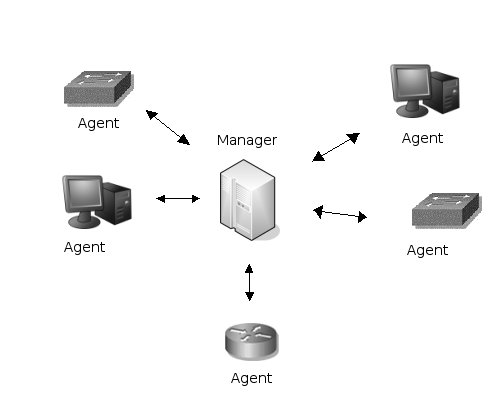
\includegraphics[width=8cm]{obrazky/02_snmp_principle.png}
		\caption{Základní princip fungování SNMP spravované sítě}
		\label{obr_snmp1}
	\end{center}
\end{figure}

\begin{itemize}
	\item \textbf{Spravovaný systém} - je zařízení (přepínač, router, atd.), na kterém je spuštěn SNMP agent. Toto zařízení shromažďuje sledované informace a pak je
	dává k dispozici manažerovi pomocí SNMP protokolu.
	\item \textbf{Agent} - je software určený pro pro správný překlad požadavků manažera a jejích vykonání na sledovaném systému. Navíc může při sledování posílat manažerovi 
	upozornění, že něco není se systémem v pořádku.
	\item \textbf{Manažer} (NMS - Network Managemet System) - je aplikace, která sleduje a spravuje všechny systémy na sledované síti. Tento systém získává od agentů data, zpracovává je do vizuální podoby, 
	čímž dává možnost administrátorovi mít přehled o celé síti. Zároveň umožňuje měnit sledované parametry přímo u agenta.
\end{itemize}

Komunikace můžeme rozdělit do dvou kategorií dle toho, kdo jí započal. Základní schéma je vyjádřeno na obrázku \ref{obr_snmp2} (\cite{tcpip_snmp}).

\begin{figure}[htp]
	\begin{center}
		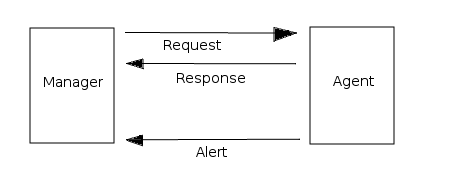
\includegraphics[width=12cm]{obrazky/02_snmp_communication.png}
		\caption{Komunikace mezi SNMP manažerem a agentem}
		\label{obr_snmp2}
	\end{center}
\end{figure}

V první části schématu je vyobrazeno standardní chování managera, který posílá dotazy agentovi, který mu odpovídá. Přesný výpis příkazů a zpráv, které si mohou tyto dva systémy mezi sebou vyměňovat, bude 
diskutován dále v této kapitole.

Druhá část schématu popisuje moment, kdy na sledovaném systému nastala nějaká extrémní situace (např. zatížení síťového spoje se blíží k maximu) a agent informuje manažera pomocí zprávi Alert (v SNMP jsou to zprávy
TRAP či INFORM, obě budoudiskutovány dále).

Je nutné zmínit, že SNMP protokol pracuje nad transportním protokolem UDP, který je nepotvrzovaný. Není tedy zaručeno, že bude komunikace probíhat bezchybně. Je možné, že některé dotazy a příkazy vůbec nedojdou
ke svému cíli, o čemž se druhá strana nikdy nedozví. Tento fakt může být překážkou při správě rozsáhlých sítí, kde jsou špatné síťové spoje.


\section{SMI, MIB standardy}
Jak již bylo zmíněno dříve, SNMP je sada standardů, která kromě komunikačního protokolu musí definovat i strukturu sledované databáze a samotná data. Tyto informace byly definovány ve standardech SMI a MIB.

\subsection*{SMI}
SMI je zkratkou pro Structure and Identification of Management Information for TCP/IP-based Internets. Tento standard (\cite{rfc1155}) popisuje a definuje základní datové struktury a typy, které protokol využívá.
Jednotlivé objekty jsou pojmenovány a organizovány, aby bylo možné k těmto datům logicky přistupovat. Dle standardu musí mít každý objekt jméno, syntaxi a kódování. Jméno jednoznačně identifikuje objekt. Datový typ
(číslo, řetězec) je určen syntaxí. Kódování zajišťuje správnou serializaci dat při přenosu mezi systémy.

Objekty, identifikovány svým jménem (OID), jsou seřazeny do hierarchické struktury. K identifikaci je použito Abstract Syntax Notation One (ASN.1). Každý OID identifikátor je složen ze skupiny přirozených čísel, které
vyjadřují jeho pozici v pomyslném stromu. Strom má kořen, který je spojen hranami s očíslovanými uzly. Každý uzel může mít vlastní děti, čímž tvoří vlastní podstrom. Takto je možno pokračovat dále do značné hloubky stromu. 
Tento standard též specifikuje, jaké identifikátory jsou přiřazeny počátku správní databáze.

\subsection*{MIB}
MIB je zkratka pro Management Information Base. Je to soubor definicí, které popisují parametry a vlastnosti sledovaného zařízení. Existuje více než 100 různých MIB, které popisují různá zařízení. Každý takovýto
soubor definic musí splňovat předpisy SMI, aby bylo zaručena správná interpretace objektů. Každý objekt (někdy také nazýván MIB objekt) je unikátně identifikován svým OID a všechny dohromady jsou uspořádány do
stromové struktury tak, jak to bylo popsáno v minulém odstavci. 

Objekty v dané databázi se dělí na \textit{skalární} a \textit{tabelární}. Skalární objekty reprezentují jeden parametr sledovaného zařízení (např. počet ethernetových karet v přepínači), kdežto tabelární objekty
jsou spojením několika spřízněných objektů (např. routovací tabulka je spojením jednotlivých záznamů, coby řádků dané tabulky).

V rámci hierarchického uspořádání jsou vyhrazeny vyšší úrovně stromu (blíže kořenu) jednotlivým standardizujícím organizacím, nižší úrovně jsou poté zadány jednotlivými společnostmi. Každý výrobce si může definovat svojí
privátní větev, do které umístí specifické informace daného zařízení.

MIB, které nebyly standardizovány a oficiálně schváleny, jsou umístěny do větve experimentální.


\section{Verze SNMP protokolu}
Celkem byly doposud standardizovány tři verze protokolu SNMP. Každá z nich definuje svoje specifické datové typy a používané datové rámce pro komunikaci. 

\subsection*{SNMPv1}
V první verzi protokolu byly definovány dvě skupiny datových typů:
\begin{itemize}
	\item Základní datové typy (Simple data types)
	\item Aplikační typy
\end{itemize}

Základní typy jsou definovány v SNMPv1 SMI a definují základní používané hodnoty:
\begin{itemize}
	\item \textbf{INTEGER} - celá čísla od $ -2^{31} $ do $ 2^{31}-1$
	\item \textbf{OCTET STRING}
	\item \textbf{OBJECT IDENTIFIER} - identifikace jednotlivých objektů v rámci normy ASN.1
\end{itemize}

Aplikační specifické typy pak jsou:
\begin{itemize}
	\item \textbf{Network Address} - obecná síťová adresa pro podporu mnoha rodin protokolů.
	\item \textbf{IpAddress} - přímo definovaný typ pro IP adresu. SMIv1 podporuje pouze 32 bitovou adresu (IPv4)
	\item \textbf{Counter} - čítač, vyjádřen celým číslem bez znaménka; Jeho hodnota se pouze zvyšuje a to až do maxima a pak se vrací zpět na nulu
	\item \textbf{Gauge} - je definována jako nezáporné celé číslo. Může hodnotu zvyšovat i snižovat a to v definovaných mezích minima a maxima
	\item \textbf{Time Ticks} - počet hodinových tiků od nějaké události, měřeno v setinách vteřiny
	\item \textbf{Opaque} - typ dovolující přenášet libovolná data v kódování ASN.1. Tato data jsou zakódována jako OCTET STRING a následně přenesena médiem.
	\item \textbf{Integers} - celočíselný typ, který předefinovává specifikaci v SMI
	\item \textbf{Unsigned Integer} - celočíselný typ bez znaménka, který stejně jako předchozí předefinovává specifikaci.
\end{itemize}

Komunikační mechanismus mezi manažerem a agentem je definován pomocí datových rámců, které je možné v rámci SNMPv1 přenášet. Tyto jsou:
\begin{itemize}
	\item \textbf{Get Request} - získání hodnoty uzlu identifikovaného OID (zpráva od manažera agentovi)
	\item \textbf{Get Next Request} - žádost o hodnotu uzlu následujícího po zaslaném OID (od manažera k agentovi)
	\item \textbf{Set Request} - Nastavení hodnoty uzlu specifikovaném OID (od manažera k agentovi) 
	\item \textbf{Get Response} - odpověď agenta manažerovi na Get a Set zprávy. Obsahují požadovanou hodnotu
	\item \textbf{Trap} - zpráva od agenta manažerovi, která upozorňuje na nastálé situace na monitorovaném systému.
\end{itemize}

Strukturu jednotlivých SNMP paketů zobrazuje obrázek \ref{obr_snmp3}.

\begin{figure}[htp]
	\begin{center}
		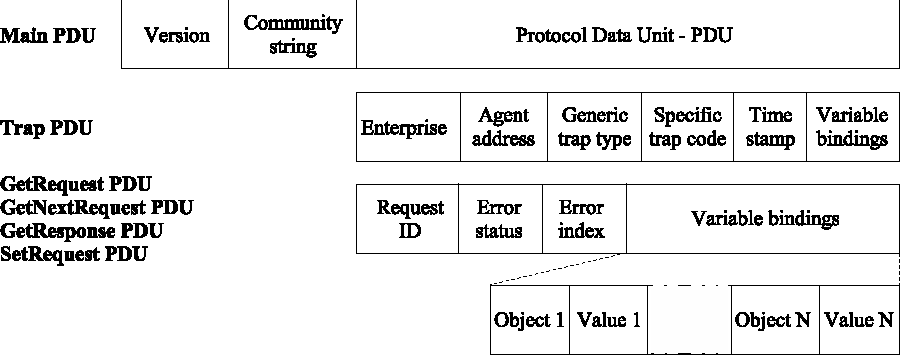
\includegraphics{obrazky/02_snmp_pdu.pdf}
		\caption{Schéma datových paketů protokolu SNMPv1 a v2 (\cite{macejko_dipl})}
		\label{obr_snmp3}
	\end{center}
\end{figure}

Hlavní část datového paketu je tvořena poli Version a Community string. První popisuje verzi SNMP protokolu použitou při komunikaci a druhé je heslo pro přístup
k položkám MIB. Blíže k bezpečnosti v dalším odstavci. Druhá část paketu se liší dle typu zprávy. Paket odeslaný agentem při výskytu monitorované události obsahuje
informace, které popisují druh problému.
\begin{itemize}
	\item \textit{Enterprise} - identifikuje typ zařízení, které zprávu poslalo
	\item \textit{Agent adress} - adresa zařízení, kde běží agent
	\item \textit{Generic trap type} - specifikuje, zda-li se jednalo o některý z předdefinovaných typů událostí (linkDown, linkUp, coldStart, aj.)
	\item \textit{Specific trap type} - identifikuje jednu z mnoha specifických událostí
\end{itemize}

Druhým typem zprávy jsou dotazy a odpovědi, které zasílá manažer a agent na ně odpovídá. Jednotlivá pole mají následující význam:
\begin{itemize}
	\item \textit{Request ID} - pořadové číslo dotazu (aby manažer věděl, na co přišla odpověď)
	\item \textit{Error status} - je nastaven pouze u odpovědi a obsahuje druh problému, který se při dotazu objevil
	\item \textit{Error index} - asociuje problém s instancí objektu.
\end{itemize}

Společným polem pro oba dva typy paketu jsou \textit{Variable bindings} - jsou to dvojice polí, kde jedna část identifikuje objekt a druhá část je jeho hodnota. Například
při dotazu příkazem GET se nastaví název objektu a v odpovědi přijde nastavena i hodnota.

Bezpečnost v této verzi protokolu je založena pouze na takzvaném \textit{community string}u, který vystupuje jako heslo. Existují pouze dvě úrovně zabezpečení
přístupu a to - pouze pro čtení (read only) a čtení-zápis (read-write access). Je patrné, že se používají pouze dvě hesla, každé pro jednu úroveň. Je to velice slabé
zabezpečení, vezmeme-li v úvahu, že toto heslo se posílá nezašifrované a každý, kdo dokáže odchytit jednotlivé pakety, si může tento řetězec přečíst. Tento nedostatek
se pokoušejí odstranit až další verze protokolu.

\subsection*{SNMPv2}
Druhá verze protokolu SNMP byla zaměřena na odstranění nedostatků verze první. Bohužel bylo vydáno několik soupeřících specifikací, označované názvy SNMPv2c, SNMPv2u, SNMPv2*, které
byly vzájemně nekompatibilní. Nicméně zlepšení oproti první verzi bylo několik. Byly definovány nové datové typy, nové zprávy a zlepšená práce s chybami.

Nové datové typy zahrnují rozšíření podpory z 32-bitových čísel na 64-bitová ( Integer32, Integer64, Counter32, ...). 

Přidané zprávy jsou:
\begin{itemize}
	\item \textbf{Get Bulk} - tento operátor se snaží efektivněji využít přenosovou kapacitu kanálu tím, že od agenta si vyžádá sérii informací pomocí jediného dotazu.
	\item \textbf{Inform} - stejná funkcionalita jako zpráva Trap ve verzi 1, ale nutné je potvrzení od manažera, že zprávu přijal (Response paket)
	\item \textbf{Response} - odpověď na předcházející Inform zprávu (od manažera k agentovi)
\end{itemize}

Ostatní zprávy SNMPv2 přebírá z předchozí verze a zachovává jejich strukturu. Stejně tak je to i s bezpečností, kde je stále použito heslo ve smyslu community stringu.

\subsection*{SNMPv3}
Třetí verze protokolu SNMP je definována sadou standardů, které nepostihují celkovou funkčnost protokolu jako takového, ale 
dodávají do systému chybějící prvky, hlavně bezpečnosti. Přímo v jednom ze standardů \cite{rfc2570} je řečeno, že tato verze může být chápána jako 
SNMPv2 s dodatečnými administrativními a bezpečnostními schopnostmi.

SNMPv3 definuje tři základní služby:
\begin{itemize}
	\item \textit{Autentifikaci} - datový přenos od manažera k agentovi může být autentifikován, aby se zajistilo ověření identity odesílajícího.
	\item \textit{Soukromí} - šifrování přenášených zpráv.
	\item \textit{Přístupová práva} - agent může definovat přístupová práva, omezovat přístup manažerům k pouze některým akcím a částem dat.
\end{itemize}

Základním principem SNMPv3 je modularita. Každá SNMP entita je tvořena SNMP řídícím systémem a vlastní aplikací. Řídící systém má za úkol 
přijímat, odesílat, šifrovat, dešifrovat všechny zprávy a dále spravuje a kontroluje monitorované objekty. Tyto funkce jsou poté k dispozici jedné či více
aplikací.

Stejně jako předchozí verze, je SNMPv3 založena primárně na transportním protokolu UDP, ale není na něj vázána. Pro přenos dat tak může být použit i jiný protokol.
Vlastní aplikační protokol SNMP je rozdělen do dvou úrovní. První zpracovává datové pakety (PDU processing layer) a druhá zpracovává zprávy (message processing layer).
Nejvyšší úroveň - PDU processing layer - se stará o zpracování příkazů (Get, Get Next, ...), které přijdou v daném paketu. Zpracovaný paket pak předá nižší úrovni - 
message processing layer - která tomuto paketu dodá hlavičku, kde jsou uložena bezpečnostní data.

Na obrázku \ref{obr_snmp4} je vyobrazen formát SNMPv3 zprávy. První část je tvořena systémem zpracování zpráv. Nese informace ohledně verzi protokolu, identifikaci zprávy,
maximální délce zprávy a nastavení bezpečnostího modelu. Druhá část je generována bezpečnostním systémem a obsahuje informace o kódování a autorizaci. Třetí část obsahuje samotná 
data.

\begin{figure}[htp]
	\begin{center}
		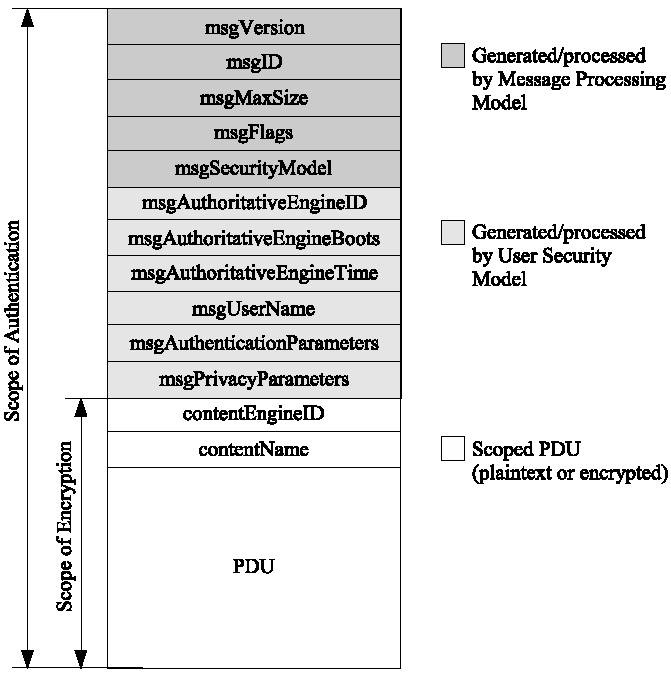
\includegraphics{obrazky/02_snmpv3_pdu.pdf}
		\caption{Schéma datového paketu protokolu SNMPv3 (\cite{macejko_dipl})}
		\label{obr_snmp4}
	\end{center}
\end{figure}


Důležitou součástí nového standardu je i systém přístupových práv (VACM - View-Based Access Control Model). Tento model umožňuje nakonfigurovat agenta tak, 
že specifickému manažerovi bude umožněn přístup pouze k části MIB. Je možné omezit manažera pro přístup pouze k části databáze monitorovaných dat a 
zároveň ještě omezit operace, které nad touto množinou může provádět. Omezení přístupu se provádí pro definované skupiny, kde součástí jedné skupiny může být
více manažerů.


\chapter{XML protokol}
\label{kap_xml}
Pan Ing. Peter Macejko ve své diplomové práci navrh systém vzdálené správy strojů pomocí komunikačního protokolu, využívajícího XML. V této kapitole budou shrnuty všechny 
navržené postupy od mapování SNMP informačního modelu až po komunikační struktury využívané správcem a spravovanými zařízeními.

\section{Obecný informační model}
Informační model je nedílnou součástí celého systému správy dat. Do něj jsou mapována veškerá monitorovaná data a jsou zde i vyjádřeny vztahy mezi daty. Ve skutečnosti
omezuje počet a druh možných dotazů. Výsledný systém, který byl pro popis jednotlivých zařízení navržen vychází z několika různých přístupů abstrakce a popisu dat.

Nejprve byla analýza problému založena na dvou možnostech - přímém mapování MIB stromu do XML dokumentu, kdy by jednotlivé uzly přesně odpovídaly MIB struktuře; objektově
orientovaném využívajícím objektové paradigma. První přístup má výhodu ve snadném převodu MIB databáze do nového formátu, ale naopak ztrácí výhodu snadné rozšiřitelnosti,
která je vlastní XML technolgoii. Problém objektového mapování je nejednoznačné rozmístění uzlů ve stromu na objekty. Takovéto mapování by bylo nutno provádět
neautomatizovaně, tj. s dopomocí člověka.

Výsledkem analýzy problému je systém využívající kousek od obou přístupů. Na nejvyšší úrovni abstrakce je každé zařízení složeno z modulů. Každý model obsahuje jistou
funkcionalitu, která je úplně oddělena od těch zbývajících. Mezi tyto moduly patří i v této práci navrhovaná brána, která propojuje zařízení bez XML podpory s ostatními
částmi sítě. V této chvíli se jedná pouze o obecný návrh každého zařízení.

\subsection{Odvození typů}
Odvozování typů je založeno na principu dědičnosti. Definice jako takové jdou od abstraktního až po detailní popis.

\subsection{Definice modulů}
Jak již bylo řečeno, každé zařízení se skládá z modulů. Jednotlivé moduly jsou též popsány XML schématem. Každé takové schéma
musí splňovat přesné požadavky na poskytované informace.

Musí být detailně popsána funkčnost, přiděleno unikátní jméno, typ a cesta ve stromové struktuře, použitá pro adresaci jednotlivých uzlů. 
SNMP moduly mají definován kořenový element, který je využit pro spojování více MIB informačních bází dohromady.

Přesný popis je možné nalézt v \cite{macejko_dipl} v kapitole 5.2.3.

\subsection{Popis zařízení}
Pro popis zařízení je využito XML schéma, stejně jako pro popis dalších částí (modulů, apod.). Na obrázku \ref{obr_xml_popis_zarizeni} je znázorněno,
jak vypadá zařízení popsané od nejvyšší úrovně. 

\begin{figure}[htp]
	\begin{center}
		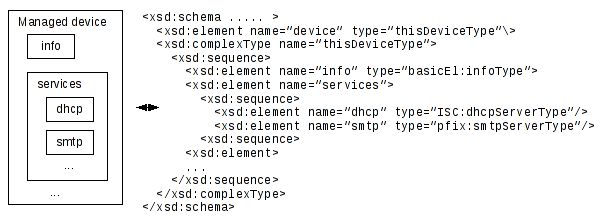
\includegraphics[width=15cm]{obrazky/03_popis_zarizeni.png}
		\caption{Popis zařízení v XML schématu (\cite{macejko_dipl})}
		\label{obr_xml_popis_zarizeni}
	\end{center}
\end{figure}

\subsection{Oznamovací zprávy}
Oznámení jsou takové zprávy, které jsou zasílány manažerovi v případě, že se na monitorovaném zařízení vyskytne nějaká událost (shodné s SNMP Trap zprávami).
V rámci SNMP jsou tyto zprávy součástí datového modelu, nicméně tyto specifické uzly MIB stromu nenesou žádná data a jsou tudíž použité pouze při generování typu
chyby či události. 

V navrženém systému jsou všechny možné upozornění (ať již předdefinované, či definované administrátorem) umístěny ve speciálním uzlu stromu \verb|notifications|, 
kde je velice jednoduché dohledat, jaké události mohou způsobit zaslání oznamuvací zprávy. Každý modul pak může mít specifikován speciální typ \verb|NotificationType|,
který popisuje právě onu událost.

\subsection{Adresace dat}
Pro adresaci dat je možno využít postupů XPath a XQuery. Jednotlivými výrazy ať už v jednom či druhém případě se bude manažer dotazovat na jednotlivé uzly v
rámci spravované databáze.


\section{Mapování MIB do XML}
V předchozí části byl rozebrán čistě obecný model popisu zařízení. Pro monitorované stroje, které nejsou kompatibilní s XML protokolem, musí existovat brána,
která bude překládat dotazy z jednoho protokolu na druhý a stejně tak i odpovědi. Je tedy nutné přesně definovat postup přepisu MIB na XML.

Je nutné vyřešit tři základní problémy - jak vyřešit importy jednotlivých MIB do sebe; jak předefinovat datové typy a jak konvertovat celý MIB strom.

\subsection{Importy}
V rámci jednotlivých MIB jsou časté odkazy na báze vyšší úrovně, kdy pak na nižších úrovních definujeme jenom část podstromu. V rámci XML budou definovány 
odkazy jako prostory jmen, které jsou odvozeny od názvu daného MIB. Odkaz na jiné schéma bude proveden použitím odkazů na typ s příslučným názvem prostoru jmen. 

\subsection{Datové typy}
V SNMP, jak bylo řečeno v předchozí kapitole, existuje několik druhů datových typů. Jednoduché (integer, string,...), aplikačně rozšířené (Gauge, IpAddress,...) a 
uživatelem definované.

Jednoduché typy budou mapovány na jejich XML ekvivalent. Na obrázku \ref{obr_xml_smi1_typy} je soupis všech aplikačně rozšířených typů a jejich popis
pomocí XML schématu (v rámci standardu SMIv1).

\begin{figure}[htp]
	\begin{center}
		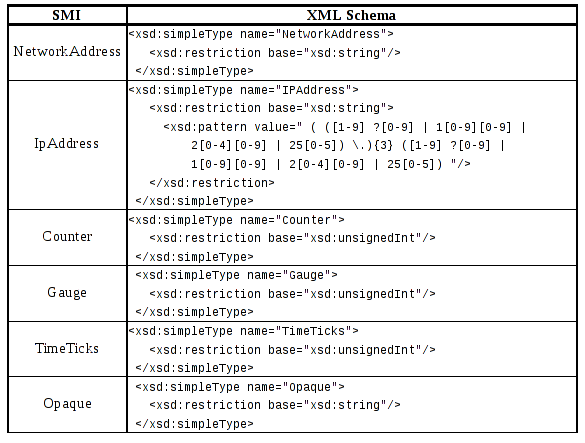
\includegraphics{obrazky/03_mapovani_smiv1.png}
		\caption{Mapování aplikačních typů SMIv1 do XML schématu (\cite{macejko_dipl})}
		\label{obr_xml_smi1_typy}
	\end{center}
\end{figure}

\begin{table}
	\centering
	{\footnotesize
	  \begin{tabular}{|p{15cm}|}
      \hline
\begin{verbatim}...
    <xsd:element name="NodeName" type="MIBName:NodeNameType"/>
...
<xsd:simpleType name="NodeNameType">
  <xsd:annotation>
    <xsd:documentation xml:lang="en">DescrText</xsd:documentation>
    <xsd:appinfo>
      <status>StatusType</status>
      <access>AccessType</access>
      <oid>AbsoluteOID</oid>
    </xsd:appinfo>
  </xsd:annotation>
  <xsd:restriction base="NodeType"/>
</xsd:simpleType>\end{verbatim}\\
      \hline
    \end{tabular}
  }
	\caption{Mapování makra OBJECT-TYPE, jednoduchý typ (SMIv1) (\cite{macejko_dipl})}
	\label{tab_xml_smi1_simple_type}
\end{table}

Součástí SMI je i možnost definovat vlastní typy. I pro tyto případy je nutno uvést definici překladu. Existují tři základní omezení při vytváření vlastních typů -
výčet, délka řetězce a rozmezí hodnot. Všechny tyto typy jsou detailně popsány a vyobrazeny v \cite{macejko_dipl}, kapitola 5.3.1.

\subsection{MIB strom}
Navržený systém využívá při mapování celého stromu oddělení definicí typů od samotné struktury stromu. Typy jsou definovány globálně a zároveň separátně od 
struktury a to z důvodu možného použití typů v rámci jiného modulu a zároveň při omezení přístupových práv do danéh oblasti stromu. V MIB jsou objekty
definovány makry (specifikované v SMI), které popisují několik základních typů uzlů. SMIv1 specifikuje OBJECT-TYPE a TRAP-TYPE makra.

OBJECT-TYPE makro definuje uzel, který obsahuje nějaká data. Může to být samotná hodnota, položka, nebo celá řádka tabulky. Mapování pak závisí na
položce \verb|SyntaxType| v samotné definici makra.

Pakliže je hodnota položky základním, rozšířeným či uživatelsky definovaným typem, bude vytvořena globální definice typu a položka bude tvořena elementem
s jednoduchým typem. Schematicky vyjádřeno v tabulce \ref{tab_xml_smi1_simple_type}.

Jestli bude hodnotou \verb|SEQUENCE|, bude vytvořen "řádkový" typ (tabulka \ref{tab_xml_smi1_sequence}).

Hodnota \verb|SEQUENCE OF| pak vyjadřuje množinu řádkových typů (tabulka \ref{tab_xml_smi1_sequenceof}).


\begin{table}
	\centering
	{\footnotesize
	  \begin{tabular}{|p{15cm}|}
      \hline
\begin{verbatim}...
    <xsd:element minOccurs="0" maxOccurs="unbounded"
             name="NodeName" type="MIBName:NodeNameType"/>
...
<xsd:complexType name="NodeNameType">
  <xsd:sequence>
    <xsd:element name="..child.." type="..childType.."/>
    ...
  </xsd:sequence>
</xsd:complexType>\end{verbatim}\\
      \hline
    \end{tabular}
  }
	\caption{Mapování SEQUENCE, makro OBJECT-TYPE (\cite{macejko_dipl})}
	\label{tab_xml_smi1_sequence}
\end{table}

\begin{table}
	\centering
	{\footnotesize
	  \begin{tabular}{|p{15cm}|}
      \hline
\begin{verbatim}...
  <xsd:element name="atTable">
    <xsd:complexType>
      <xsd:sequence>
        <xsd:element ..SEQUENCE.. />
      </xsd:sequence>
    </xsd:complexType>
  </xsd:element>
...\end{verbatim}\\
      \hline
    \end{tabular}
  }
	\caption{Mapování SEQUENCE OF, makro OBJECT-TYPE (\cite{macejko_dipl})}
	\label{tab_xml_smi1_sequenceof}
\end{table}

Dalším typem objektu jsou upozornění definované pomocí TRAP-TYPE makra. Tyto definují uzly bez hodnot, pouze specifikují danou událost. V navrženém systému
tedy nemusí být součástí stromu, ale pouze globálních typových definicí. Bude použit jednoduchý typ popisující čas a den (datetime type) se speciálním elementem
v části \verb|appinfo|.

\begin{table}
	\centering
	{\footnotesize
	  \begin{tabular}{|p{15cm}|}
      \hline
\begin{verbatim}<xsd:simpleType name="NodeNameType">
  <xsd:annotation>
    <xsd:documentation xml:lang="en">DescrText</xsd:documentation>
    <xsd:appinfo>
      <enterprise>EnterpriseName</enterprise>
      <variable>VariableType</variable>
      <reference>ReferenceType</reference>
      <trapNumber>TrapNumber</trapNumber>
    </xsd:appinfo>
  </xsd:annotation>
  <xsd:restriction base="xsd:dateTime"/>
</xsd:simpleType>\end{verbatim}\\
      \hline
    \end{tabular}
  }
	\caption{Mapování TRAP-TYPE makra (\cite{macejko_dipl})}
	\label{tab_xml_trap_type}
\end{table}

\newpage

\section{Zprávy}
Navrhovaný systém by měl využívat spolehlivého a potvrzovaného přenosového protokolu, na rozdíl od nepotvrzovaného SNMP. Zaroveň by mělo být možno
přenášet zprávy v co nejjednodušším formátu. Proto bylo rozhodnuto o použití protokolu HTTP, který využívá přenosový protokol TCP, čímž je zajištěn 
splehlivý přenos. Všecha data se budou přenášet pomocí HTTP zprávy POST.

HTTP je bezestavový protokol. Veškerá komunikace se sestává z dvojice dotaz a odpověď. Na serveru se neudržují jakékoliv další informace ohledně probíhajícím
spojení. Tato nenáročnost dovoluje implementaci na velice různorodém hardwaru.

Bezpečnost přenosu může být řešena za použití tunelování paketů (IPSec, STunel,...), nebo je možno využít výhody HTTPS (HTTP over SSL). 

Veškerá přenášená data budou ve formátu XML dokumentu s kořenovým uzlem \verb|message|. Tento uzel má několik atributů, které specifikují jeho zpracování a přístupová
práva. Jsou to \verb|queue|, \verb|password|, \verb|context|. První atribut určuje frontu (může být založeno na prioritním zpracování), ve které bude požadavek zpracován.
V principu ale nejsou agenti ani brány povinni takovouto funkčnost implementovat. Zprávy pak budou zpracovány sekvenčně a odpovědi budou generovány v přesném pořadí tak, 
jak přišly dotazy. Zbylé dva atributy slouží pro vymezení přístupu uživatele (\verb|context|) na určitý podstrom dat. 

Bylo již naznačeno, že zpráva může obsahovat několik jednotlivých dotazů. Struktura zprávy je vyjádřena na obrázku \ref{obr_xml_struktura_zpravy}.

\begin{figure}[htp]
	\begin{center}
		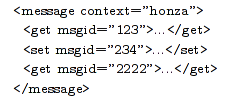
\includegraphics{obrazky/03_struktura_zpravy.png}
		\caption{Struktura XML zprávy}
		\label{obr_xml_struktura_zpravy}
	\end{center}
\end{figure}

Dotazy a odpovědi, které definují komunikaci mezi manažerem a klientem, jsou popsány níže. Přesné XML schéma definující úplnou strukturu zpráv obsahuje (\cite{macejko_dipl}, příloha D).

\subsubsection*{DISCOVERY}
Tato zpráva je první, kterou zašle manažer agentovi, aby zjistil, jaká monitorovaná data jsou k dispozici.
Povinným atributem je číslo verze protokolu (\verb|protocolVersion|) a nepovinným je \verb|fullDescription| pro bližší specifikace
typů spravovaných dat.

\begin{verbatim}
<message context="honza">
  <discovery protocolVersion="1.0" msgid="123" />
</message>
\end{verbatim}

\subsubsection*{PUBLICATION}
Agentova odpověď na manažerův dotaz DISCOVERY. V rámci zprávy je uvedeno, jakou verzi protokolu agent používá a jaká data spravuje. Tato data jsou pak
manažerem zpracována a použita jako informační model.

\begin{verbatim}
<publication msgid="123">
  <info>
    <xpath>1.0</xpath>
    ...
  </info>
  <dataModel>
    ... XML schema popisující spravovaná data ...
  </dataModel>
</publication>
\end{verbatim}

Pakliže agent nepodporuje danou verzi protokolu, musí odpovědět chybovou zprávou:

\begin{verbatim}
<publication msgid="123">
  <error code="1">Protocol not supported</error>
</publication>
\end{verbatim}

\subsubsection*{GET}
Tímto dotazem se manažer ptá agenta na hodnotu nějakého uzlu. Pro specifikaci jakého je nutno použít XPath či XQuery.

\begin{verbatim}
<get msgid="123">
  <xpath>
    device/data/interface
  </xpath>
</get>
\end{verbatim}


\subsubsection*{SET}
Zpráva SET je určena pro nastavení hodnoty uzlu. Struktura je podobná zprávě GET, ale obsahuje navíc element \verb|value|.

\begin{verbatim}
<set msgid="123">
  <xpath>
    device/data/interface/status
  </xpath>
  <value>4</value>
</set>
\end{verbatim}

\subsubsection*{RESPONSE}
Odpověď na zprávy GET a SET. V případě GET nese zpráva příslušná data. Pakliže je to odpověď na SET, je to pouze potvrzení, že hodnota byla uzlu úspěšně nastavena.

\begin{verbatim}
<response msgid="123">
  <value>4</value>
</response>

<response msgid="123" />
\end{verbatim}

\subsubsection*{EVENT}
Pro oznamování asynchronních událostí, je tu zpráva EVEN (stejná funkcionalita jako TRAP u SNMP). Přenášené informace specifikují, která událost vyvolala toto oznámení,
kdo to poslal, datum a čas, případně nějaká další data, která by mohla být při řešení problému užitečná.

\begin{verbatim}
<event msgid="123" timestamp="" senderID="router1" eventSpec="/device/notifications/dhcp/noFreeLease">
  <data>
    <value valueLocation="/data/services/dhcp/leases/free">0</value>
    <value valueLocation="/data/services/dhcp/leases/used">50</value>
  </data>
</event>
\end{verbatim}

Je nutné, aby doručení této zprávy bylo potvrzeno. Což bude dodrženo použitým protokolem.

\subsubsection*{SUBSCRIBE}
Touto zprávou se manažer přihlásí k opakovanému zasílání dat. Potvrzením je pak první doručení dat - zpráva DISTRIBUTION - nebo chybové zprávy, že je něco v nepořádku.
Je možné specifikovat ještě nepovinný atribut \verb|frequency| - doba ve vteřinách, po které mají být opakovaně zasílány zprávy. Další nepovinné atributy \verb|distrid| a \verb|delete|
jsou využity pro editaci či smazání daného přihlášení.

\begin{verbatim}
<subscribe msgid="123" frequency="150">
  <xpath>/device/data/interface/status</xpath>
</subscribe>
\end{verbatim}

\subsubsection*{DISTRIBUTION}
Zpráva obsahuje data, o která si manažer řekl. Je nutné, aby odesílaná data byla ve stejném pořadí, ve kterém byla ve zprávě SUBSCRIBE. 
Povinný atribut \verb|distrid| je určený k identifikaci příchozích dat u manažera.

\begin{verbatim}
<distribution msgid="123" distrid="5678">
  <value>1</value>
  <valuea>500</value>
</distribution>
\end{verbatim}

Příjem těchto dat je též nutné potvrdit, což zajistí transportní protokol.




\chapter{Návrh systému}
\label{kap_navrh_systemu}
V předchozích dvou kapitolách byla rozebrána teoretická část problému. V této kapitole shrneme požadavky vyplývající z teorie, které je nutno zakomponovat do
výsledného systému. Nejprve bude schématicky vyjádřena obecná funkcionalita systému, která se následně bude rozebírat detailněji.

\section{Teoretické požadavky}
Nároky na systém, které vyplývají z teorie můžeme rozdělit do třech částí - implementace SNMP protokolu, implementace navrženého XML protokolu a propojení těchto dvou protokolů dohromady.

Hlavním požadavkem, který vyplývá i ze zadání práce, je vytvořit modulární systém, který bude nejenom spojovat současné verze protokolů, ale bude počítat i s potenciálním rozšířením do
budoucna. Obecné schéma navrhovaného systému zobrazuje obrázek \ref{obr_an_obecne_schema}. 

\begin{figure}[htp]
	\begin{center}
		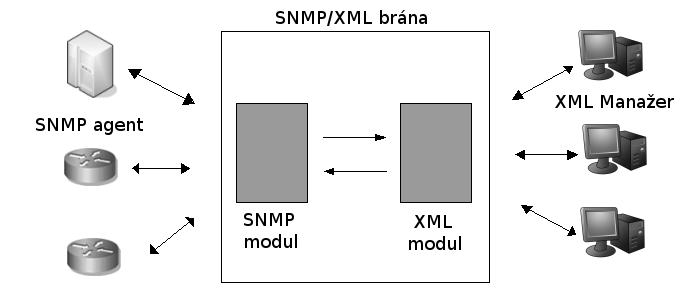
\includegraphics[width=15cm]{obrazky/04_obecne_schema.png}
		\caption{Schéma navrhovahého systému}
		\label{obr_an_obecne_schema}
	\end{center}
\end{figure}

Zde je vidět, že oba dva protokolové moduly jsou na sobě nezávislé a jejich interakce spočívá v předávání si zpráv. Nyní přejděme k detailnějším požadavkům na výše zmíněné části systému.

V rámci \textit{SNMP protokolu} je požadováno
\begin{itemize}
	\item implementace komunikačních struktur protokolů SNMPv1 a SNMPv2
	\item převzetí bezpečnostního schématu z tohoto protokolu
\end{itemize}

\textit{XML orientovaná část programu } má za úkol
\begin{itemize}
	\item implementovat komunikační struktury navrženého protokolu
	\item navrhnout efektivní správu XML struktur v paměti
	\item poskytnout XML manažerům transparentní získání dat z monitorovaných zařízení
	\item mapovat rozšířenou množinu funkcí v rámci XML protokolu do SNMP
	\item s manažery komunikovat pouze přes HTTP/HTTPS protokol
\end{itemize}
Spojením protokolů je myšlen přechod od databázových struktur jednoho protokolu k druhému. V našem případě je to transformace SNMP MIB do XML, jak bylo vysvětleno v kapitole \ref{kap_xml}.

\subsection{XML}
Nejprve se zaměříme na reprezentaci dat, které budou v rámci XML popisovat jak bránu, tak monitorované zařízení. Z předchozích kapitol vyplynulo, že bude použito částečně objektového přístupu a přímého mapování MIB.
Strukturu dat bude popisovat XML dokument, strom, který má strukturu vyjádřenou na obrázku \ref{obr_an_strom_struktura}.

\begin{figure}[htp]
	\begin{center}
		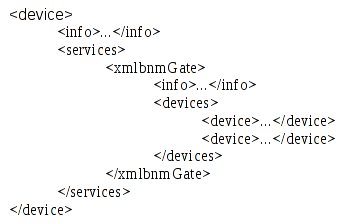
\includegraphics{obrazky/04_schema_dokumentu.png}
		\caption{Obecná struktura XML dokumentu}
		\label{obr_an_strom_struktura}
	\end{center}
\end{figure}

\begin{figure}[htp]
	\begin{center}
		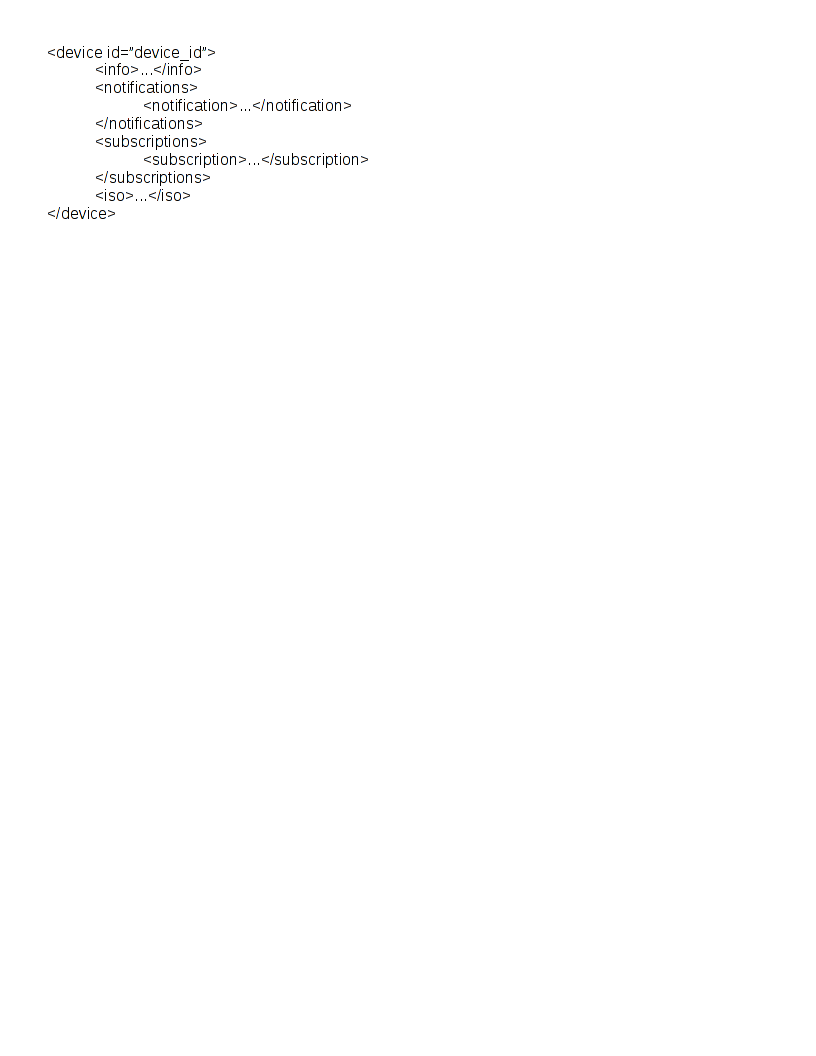
\includegraphics{obrazky/04_schema_device.png}
		\caption{Struktura elementu device}
		\label{obr_an_device_struktura}
	\end{center}
\end{figure}

Kořenový uzel specifikuje celé zařízení vystupující jako protokolová brána, obsahuje tyto elementy:
\begin{itemize}
	\item \textbf{info} - tento element obsahuje text, kterým je popsáno dané zařízení.
	\item \textbf{services} - element vymezující poskytované služby (při širší implementaci může obsahovat služby DNS, DHCP, apod.)
	\item \textbf{xmlbnmGate} - naše služba poskytující spojení XML a SNMP protokolu
	\item \textbf{device} - je podelementem \textbf{xmlbnmGate} a vymezuje jedno monitorované zařízení
\end{itemize}

Prvky \textbf{device} jsou do XML dokumentu přidávány na základě informací v konfiguračním souboru (viz kapitola \ref{sec_an_struktura_programu}).

Strukturu elementu \textbf{device} popisuje obrázek \ref{obr_an_device_struktura}. Každý takovýto element bude obsahovat následující informace:
\begin{itemize}
	\item \textbf{info} - stejně jako kořenový element popisuje dané zařízení
	\item \textbf{notifications} - obsahuje elementy a typy upozornění (TRAP zprávy v rámci SNMP), na které manažer čeká
	\item \textbf{subscriptions} - obsahuje informace o datech, které si nechává manažer posílat v pravidelných intervalech (více v popisu komunikace)
	\item \textbf{data} - sem jsou mapována veškerá data přímo z MIB.
\end{itemize}

Samotný element má atribut \textit{id}, což je jeho identifikace v rámci xml dokumentu. Dle tohoto unikátního čísla je pak možné
v sadě dotazů rozpoznat, ke kterému zařízení se dotaz vztahuje.


Element \textbf{info} obsahuje elementy, které specifikují jméno a popis zařízení (viz obrázek \ref{obr_an_info_element}).

\begin{figure}[htp]
	\begin{center}
		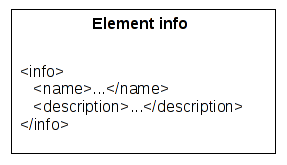
\includegraphics{obrazky/04_element_info.png}
		\caption{Struktura elementu info}
		\label{obr_an_info_element}
	\end{center}
\end{figure}

Jednotlivé podelementy uzlu \textbf{subscriptions} musí z podstaty věci obsahovat informace, které určují, jaké objekty chce manažer pravidelně sledovat, identifikovat
manažera, aby mu mohly být data doručena a specifikovat časový interval, tj. frekvenci sledování příslušné veličiny.

Děti uzlu \textbf{notifications} určují, které typy událostí jsou sledovány u daného zařízení. V rámci konfigurace systému je nezbytné, aby pro každé zařízení
bylo jasně definováno, kam mají být příslušné zprávy o událostech zasílány. Tudíž v rámci typu události je nutné uvést příjemce, který bude zprávy očekávat. Přesná 
specifikace jednotlivých uzlů dokumentu je v příloze 
%TODO dopsat referenci na prilohu, kde jsou specifikace jednotlivych uzlu

Mapování dat z MIB bylo obecně popsáno v kapitole \ref{kap_xml} a přesný algoritmus bude specifikován v následující kapitole. Pro adresaci jednotlivých objektů
je, jak bylo již nastíněno v předchozí kapitole, použito mechanismů XPath či XQuery. Dotaz na položku z MIB může vypadat následovně
\begin{verbatim}
	/device/services/xmlbnmgate/device[id=1]/data/...
\end{verbatim}

\subsubsection*{Zprávy}
Zprávy, které budou posílány mezi manažerem a bránou, mají formu XML dokumentu. Schématicky je znázorněna a popsána v kapitole \ref{kap_xml}, obrázek .
%TODO dodat cislo obrazku odkazujici na message format v ramci xml kapitoly

Kořenový element message obaluje veškerá posílaná data. Může obsahovat několik dílčích dotazů, nastavení a ostatních informací, které budou vykonávány postupně
jedna po druhé. V rámci teorie byla nastíněna možnost použití několika různých front, které by byly specifikovány identifikátorem a zaručovaly by různou
prioritu zpracování. Navrhovaný systém bude podporovat pouze jednu frontu zpracování zpráv, čímž budou jednotlivé dotazy zpracovány postupně. Bude tak zaručena
integrita dat a předejde se různým extrémním situacím.

Komunikace mezi manažerem a bránou je na XML úrovni omezena na zprávy
\begin{itemize}
	\item Get
	\item Sset
	\item Discovery
	\item Publication
	\item Subscription
	\item Distribution
	\item Event
\end{itemize}

Přesná struktura a popis funkce jednotlivých zpráv byla popsána v předchozí kapitole.


\subsubsection*{Komunikační protokol}
Od protokolu SNMP se XML část komunikace liší taky tím, že bude probíhat na spolehlivém a potvrzovaném protokolu - HTTP. Každá zpráva, která
je poslána, musí mít potvrzeno doručení, což tento aplikační protokol, využívající transportního protokolu TCP, nabízí. 

Informace budou posílány ve formátu HTTP POST zprávy. Strukturu dotazu a odpovědi zobrazuje obrázek \ref{obr_an_http_post} a komunikaci obrázek \ref{obr_an_http_request}.

\begin{figure}[htp]
	\begin{center}
		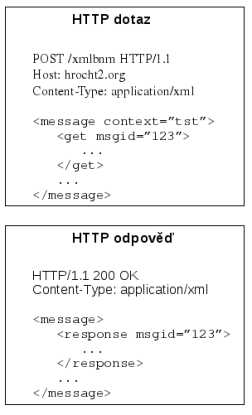
\includegraphics{obrazky/04_http_post.png}
		\caption{HTTP zprávy předávané mezi manažerem a bránou}
		\label{obr_an_http_post}
	\end{center}
\end{figure}

\begin{figure}[htp]
	\begin{center}
		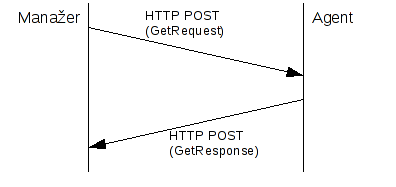
\includegraphics{obrazky/04_http_request.png}
		\caption{HTTP komunikace mezi manažerem a agentem/bránou}
		\label{obr_an_http_request}
	\end{center}
\end{figure}

%TODO: dodelat schema posilani dotazu a odpovedi. Tento obrazek je moc malej, aby byl sam na cele strance.

Otázka bezpečného přenosu dat byla řešena v předchozí kapitole a byl zvolen protokol HTTPS. Zajištění distribuce a zpracování certifikátů bude
diskutováno dále v této kapitole.


\subsection{SNMP}
Druhou část komunikace tvoří SNMP protokol. Z kapitoly \ref{kap_snmp} vychází seznam zpráv, které je nutné implementovat:
\begin{itemize}
	\item Get
	\item Set
	\item Response
	\item GetNext
	\item Trap
\end{itemize}

V rámci komunikace se v naší práci budeme zaobírat verzemi SNMPv1 a SNMPv2. Samotná implementace a mapování SNMP zpráv na XML dotazy
bude diskutována až v kapitole \ref{kap_implementace}.

Bezpečnost se v SNMP omezuje pouze na komunitní heslo, které je zasíláno jako součást XML zprávy a bude pouze přepsáno do SNMP paketu. 
Je tedy zřejmé, že ponecháváme bezpečnost takovou, jak je standardizována v SNMP protokolu.


\section{Struktura programu}
\label{sec_an_struktura_programu}
Před samotným návrhem jednotlivých funkčních elementů je nutno zvolit, jak bude program fungovat a jevit se globálně. Vzhledem k
nabízeným službám a komunikaci, je možné zvolit koncepci podobnou webovým službám (založených na principu SOAP). Druhým možným přístupem je zvolit
na pozadí běžící aplikaci - démona, který bude po celou dobu svého běhu monitorovat a zpracovávat příchozí požadavky.

\subsection{SOAP vs. démon}
Kompozice struktury jako webové služby založené na SOAP architektuře má několik předností. Je tím hlavně přenositelnost a jednoduchost nasazení. Vše, co je potřeba k běhu,
je aplikační server. Nainstalování a spuštění služby je již pak otázkou okamžiku. Samotná struktura kódu je též o něco jednodušší, než v případě démona. Je nutné se starat pouze o
příchozí požadavek a jeho zpracování.

Bohužel tento přístup má ale i mnoho nevýhod. Zaprvé je to reakční doba, za kterou je systém schopen zaslat manažerovi odpověď. Pro samotné zpracování požadavku
je nutno v paměti (či v souboru) udržovat XML reprezentaci MIB tak, jak bylo popsáno dříve. Při použití tohoto postupu se po každém přijatém požadavku musí načíst informace ze souboru
a teprve poté je možno data zpracovat.

Dalším sporným bodem je periodické zasílání zpráv manažerům, kteří o to požádali zprávou Subscription. V takovém případě musí běžet jeden proces, který v určených intervalech zasílý SNMP
dotazy na monitorované zařízení, což je neslučitelné se základní myšlenkou webových služeb.

Asi největší nevýhodou tohoto přístupu je transformace dat z MIB do XML. Při spuštění webové služby je nutné, aby již všechna zařízení měla své monitorované informace uloženy v XML formátu, 
protože při požadavku již není čas data transformovat. Tento akt by musel být od služby oddělen a buď svěřen periodicky se spouštěnému skriptu, nebo by jej administrátor musel provést pokaždé,
když se změní počet, druh či monitorované údaje jednotlivých zařízení.

Oproti tomu stojí druhý přístup - strukturovat aplikaci jako démona. Je pravdou, že výsledný kód aplikace je složitější, přenositelnost horší a není zde možné mluvit o platformové nezávislosti (co se implementace v C++ týče).
Nicméně získáme tím výhodu v podobě relativně malé reakční doby, protože veškeré informace jsou za běhu uloženy v operační paměti a není je nutno načítat z pevného disku. Systém periodického monitorování
zařízení může být jednoduše spravován jedním vláknem procesu, zatímco ostatní vlákna se starají o příchozí a odchozí požadavky. Transformace dat pak může být bez úhony součástí samotného programu.

\subsection{Navrhovaná aplikace}
Fáze běhu navrhovaného systému zobrazuje diagram na obrázku \ref{obr_an_beh_programu}.

\begin{figure}[htp]
	\begin{center}
		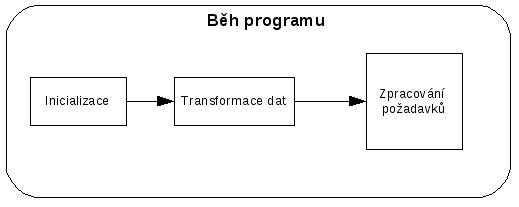
\includegraphics{obrazky/04_beh_programu.png}
		\caption{Fáze běhu programu}
		\label{obr_an_beh_programu}
	\end{center}
\end{figure}

\subsubsection{Inicializace}
V první, inicializační, fázi je načten konfigurační soubor, jehož specifikace bude popsána v kapitole \ref{kap_implementace}. Tento soubor obsahuje veškeré informace o monitorovaných zařízeních, stejně tak
jako základní nastavení protokolové brány. Každé zařízení musí mít definováno SNMP spojení (adresu), seznam MIB, které vyjadřují všechny nabízené informace. Dále bude obsahovat nastavení ohledně 
asynchronních událostí a jakému manažerovi je nutno je přeposílat. Důležitým nastavením je i verze SNMP protokolu, jakou zařízení podporuje.

Protokolová brána bude mít sama o sobě speciální část, která bude definovat komunikační porty, na kterých budou přijímány a zpracovávány požadavky, cesty k různým logovacím souborům a cesty k adresáři s MIB a XML soubory.

Součástí inicializace je i ověření, zda-li všechna monitorovaná zařízení fungují. Pakliže některé nebudou funkční, systém je ze seznamu vyškrtne a nebude je nabízet manažerům ke správě.

\subsubsection{Transformace dat}
Transformace dat představuje samotné mapování MIB do XML tak, jak bylo popsáno dříve. Pro každé zařízení může být specifikováno několik různých MIB, jak veřejné, tak proprietární. Pro každé
zařízení je tedy nutno vytvořit XML dokument, popisující veškeré MIB informace.

V tomt místě jsou možné dvě cesty, jak vybudovat výstupní XML dokument. Jednou možností je zahrnout veškeré informace o všech zařízeních do jednoho souboru, který potom bude rozesílán každému manažerovi, jenž si o něj řekne. Tato varianta
je sice praktická, ale neefektivní. Pro zařízení s velkým množstvím informací by byl výsledný dokument opravdu veliký. Kdyby manažer chtěl spravovat pouze jediné zařízení, byl by stejně nucen stáhnout velký objem dat, než
by mu bylo dovoleno pracovat dále.

Proto bude použito následujícího schématu. Systém bude při prvním kontaktu s manažerem publikovat pouze informace týkající se počtu a typu zařízení, které spravuje. Jednotlivá zařízení budou mít svůj samostatný soubor
s daty. Manažer si pak bude moci zvolit pouze určitá data, která ho zajímají. Tím se velmi sníží počáteční zatížení linky.

\subsubsection{Zpracovávání požadavků}
Po úspěšném přůchodu oběma přechozími fázemi se program dostává do situace, kdy vyčkává na příchozí požadavky, ať již ze strany manažera či SNMP zařízení.

Jak již bylo popsáno na začátku této kapitoly, o komunikaci se starají dva moduly - SNMP a XML. Proto taky komunikační rozhraní se dělí na dvě části.

SNMP modul bude komunikovat pomocí protokolu UDP, posíláním SNMP zpráv. Tato část rozhraní bude blíže popsána v následující kapitole.

Komunikace v rámci XML je na bázi HTTP protokolu. Pro zpracování mnoha požadavků, které je nutno očekávat, bude použito HTTP serveru. V tomto případě se nám nabízí dvě možnosti
řešení - využijeme nějakého již stávajícího webového serveru (Apache, Tomcat, ...), na kterém budeme spouštět CGI script a tak komunikovat s naším programem, nebo do aplikace nějaký jednoduchý server
naimplementujeme. Výhodou již existujícího řešení by byla pouhá konstrukce komunikačního kanálu mezi protokolovou branou a zmíněným serverem. Je ale pravděpodobné, že bude potřeba mít větší kontrolu
nad přijímanými a odesílanými zprávami, což vlastní implementovaný server poskytuje. Přednostně tedy bude vybrána varianta s embedded HTTP serverem.

Ve spojitosti s protokolem HTTP je nutné zmínit použití certifikátů pro zabezpečený přenost a použití protokolu HTTPS. Pakliže by bylo využito externího webového serveru, bude ponechána
veškerá zodpovědnost a konfigurace na administrátorovi serveru, který se bude muset postarat o obdržení a distribuci certifikátu. Jestli bude server součástí protokolové brány, bude
nutno přiložit certifikát k aplikaci a v konfiguračním souboru zajistit jeho použití.

\section{Správa protokolové brány}
V rámci spravovaných zařízení se naskýtá otázka, jestli by bylo možno spravovat i samotnou bránu přes navržený XML protokol (je myšlena aplikace jako taková). 

Navržený systém tuto skutečnost neumožňuje. Samotná brána nebude vykazovat vlastnosti agenta. Ke správě stroje, na kterém brána poběží, bude nutné použít XML či SNMP agenta, který tuto 
funkcionalitu bude zajišťovat. Je možné pak v konfiguračním souboru nastavit, aby brána nabízela komunikaci se SNMP agentem na tomtéž stroji. XML agent bude komunikovat s manažerem přímo na definovaném portu.
Implementace takvého agenta ale již přesahuje rámec této práce.

Správa aplikace je pak omezena pouze na konfigurační soubor a bude ji nutné při každé změně restartovat (jak je tomu například i u konfigurace webových serverů). Je to z důvodu zachování integrity poskytovaných dat.
Při změně informačních bází jednotlivých zařízení, přidání či odebrání monitorovaných strojů, je nutno přegenerovat všechny XML dokumenty, které jsou pak distribuovány manažerům. Nekorektnost dat, které manažer obdržel a které
by byly aktuální, kdyby se změnily za plného provozu, by mohla mít pak vážné následky na data, která by manažeři dostali zpět.

\section{XML manažerská aplikace}
Součástí této práce je i implementace základního XML manažera tak, aby dovolil ukázat veškeré funkční aspekty protokolové brány.

Program bude mít implementován celý XML komunikační protokol tak, jak byl navržen v kapitole \ref{kap_xml}. Tudíž základní příkazy - Discovery, Publication, Get, Set, Subscription, Distribution.

Správu monitorovaných zařízení zahajuje komunikací buď přímo s agentem či bránou. Vyžádá si od nich 
dokument, který popisuje nabízené informace. Pakliže se jedná o komunikaci s bránou, tak nejprve zjistí, jaká zařízení jsou k dispozici a pak si některé vybere a teprve pak požádá o jejich XML popis dat.
Algoritmus budování XML stromu použitelného pro další interakci se zařízeními je stejný jako v případě brány a bude popsán v další kapitole. 

Aplikace bude napsána v jazyce C++ stejně jako protokolová brána. Využití podpory grafického rozhraní je možné.








\chapter{Implementace}
\label{kap_implementace}

Vlastní implementace protokolové brány je v této kapitole vysvětlena v rámci několika částí. Nejprve je popsána
struktura programu, popis tříd, jejich vztah mezi sebou a hlavní funkce, kterou plní. Následuje přehled všech použitých knihoven pro
lepší pochopení dalšího popisu funkce aplikace. Další část tvoří vysvětlení výkonného cyklu programu krok za krokem od spuštění až po
zpracování jednotlivých zpráv. Jsou vysvětleny dosažené výsledky při paměťové optimalizaci a detailně rozebrán systém komunikačních front.
Jako poslední je popsán XML manažer, který byl navržen v předchozí kapitole.

\section{Třídy, vlastnosti a jejich vztahy}
Jak bylo předesláno v předchozí kapitole, při tvorbě byl dáván velký důraz na modularitu jednotlivých součástí programu.
V praxi to znamená, že jednotlivé komunikační jednotky brány nemají tušení, jak ta druhá provádí konkrétní
operace, ale jediným spojením jsou přesně definované struktury obsahující veškeré nutné informace.

Strukturu programu tvoří čtyři třídy:
\begin{itemize}
	\item \textbf{SnmpXmlGate} - hlavní třída, která ovládá běh programu. Při spouštění inicializuje veškeré datové struktury,
	připraví oba komunikační moduly a předá jim řízení.
	\item \textbf{SnmpModule}  - komunikační modul pro zpracování veškerých SNMP požadavků. Plní dvě funkce. První je získávání dat
	z agentů v reakci na dotaz od manažera (resp. XML modulu). Druhou je zpracování asynchronních událostí (Trap, Notification), které
	se na agentech vyskytnou a získané informace zašle definovaným manažerům.
	\item \textbf{Mib2Xsd}	   - transformační třída pro překlad MIB databáze do XML schématu. Netvoří však jenom tento popis, ale zároveň 
	i vytváří finální XML dokument, se kterým pak hlavní program pracuje.
	\item \textbf{XmlModule}   - druhý komunikační modul pro zpracování XML požadavků. Tato třída je vlastní implementací
	navrženého XML protokolu a je pro tuto práci stěžejní.
\end{itemize}

Vzájemné vztahy těchto tříd jsou vyjádřeny na obrázku \ref{obr_impl_vztahy_trid}.

\begin{figure}[htp]
	\begin{center}
		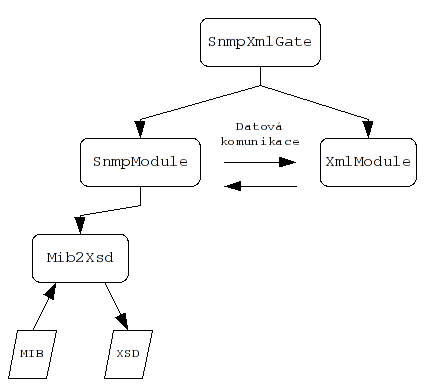
\includegraphics[width=12cm]{obrazky/05_schema_trid.png}
		\caption{Schéma tříd aplikace}
		\label{obr_impl_vztahy_trid}
	\end{center}
\end{figure}


\section{Použité knihovny}
Při tvorbě programu bylo použito několik knihoven, které zajišťují bezproblémový chod aplikace.

%TODO: reference na jednotlive knihovny
\begin{itemize}
	\item \textbf{ \textit{Xerces-C++ a Xalan-C++} } - knihovny zajišťující manipulace s XML dokumenty, vyhledávání pomocí XPath výrazů.
	\item \textbf{ \textit{Net-SNMP} } - knhovna napsaná v jazyce C, určená pro interpretaci a manipulaci s daty MIB databází, zasílání a 
	přijímání datových SNMP paketů.
	\item \textbf{ \textit{libMicroHTTPD} } - volně dostupný HTTP server s podporou použití SSL protokolu při spojení.
	\item \textbf{ \textit{libCUrl} } - volně dostupná knihovna určená pro klientskou stranu spojení. Podporuje mimo jiné protokoly HTTP, FTP a
	umožňuje použít i SSL certifikáty pro zabezpečení daného spojení.
\end{itemize}

Knihovny Xerces, Xalan, libCUrl a libMicroHTTPD využívá XML modul, který má na starosti běh HTTP serveru, operace s XML dokumenty a periodické zasílání
informací.

SNMP modul využívá knihoven Net-SNMP a libCUrl. Druhou jmenovanou využívá vlákno pro zpracování asynchronních událostí (viz dále v této kapitole).


\section{Popis výkonného cyklu}
Detailní popis funkcí jednotlivých tříd je součástí popisu fungování protokolové brány. Jak bylo napsáno v předchozí kapitole,
v rámci běhu programu je několik přesně definovaných fází, ve kterých se systém může nacházet. Tyto jsou vyobrazeny na obrázku \ref{obr_an_beh_programu}.
Některé z těchto fází byly oproti návrhu lehce pozměněny, či rozšířeny, dle potřebného rozsahu splňovaných funkcí.

\subsection{Inicializační fáze}
Je důležité připomenout, že již v návrhu bylo stanoveno, jako optimální řešení, že program bude běžet jako démon. Tomu odpovídá
i manipulace s programem. Byl vytvořen spouštěcí skript, který ovládá běh programu - spouští, zastavuje či restartuje (popis instalace,
struktura spouštěcího skriptu a použití je v příloze \ref{kap_uzivatelska_prirucka_brana}).
Jediným vstupním parametrem systému je konfigurační soubor, který je formátován jako dokument XML (přesná struktura souboru se všemi 
povolenými a nutnými elementy je v příloze \ref{kap_struktura_conf_souboru}). Tento obsahuje veškeré nutné informace pro běh systému.

\subsubsection*{Konfigurační soubor}
Informace jsou strukturovány do elementů, kdy každý popisuje jedno spravované zařízení. Každé zařízení je nutné identifikovat
unikátním číslem, které bude použito později při komunikaci s manažery. Dále je nutné specifikovat SNMP přístupové informace
k agentovi:
\begin{itemize}
	\item IP adresu či url
	\item verzi SNMP protokolu
	\item MIB báze, které popisují zařízení
	\item přístupová hesla (community string) pro zápis a čtení
\end{itemize}

Poslední položkou, která je čistě volitelná, je možné definovat manažery, kteří obdrží informace o asynchronních událostech. Každý 
manažer je definován IP adresou či url a portem, na který se budou zasílat jednotlivé zprávy.

Specifickým elementem je definice samotné brány. Tento element obsahuje veškeré informace výše popsány, ale jsou přidány ještě povinné elementy:
\begin{itemize}
	\item \textbf{logFile} - identifikuje soubor, do kterého budou ukládány veškeré textové výstupy.
	\item \textbf{snmp}    - obsahuje informace o cestě k souborům definujícím MIB databáze a portu, na kterém budou poslouchány asynchronní události
	\item \textbf{xml}     - definuje xml modul systému. Je zde verze XML protokolu; přístupová práva pro čtení a zápis; cesta k ukládání XSD popisu zařízení;
	porty pro poslouchání požadavků a odesílání odpovědí.
	\item \textbf{security} - obsahuje případné informace o certifikátu a klíči použitém při přístupu přes protokol HTTPS.
\end{itemize}

\subsubsection*{Zpracování a ověření informací}
Poté, co je bezchybně zpracován vstupní soubor, je přistoupeno ke zpracování informací ohledně jednotlivých zařízeních. Tuto fázi má
na starosti třída \textit{SnmpModule}. Nejprve je ověřeno, jestli dané zařízení vůbec funguje a je na něm přítomen SNMP agent. Odešle
se tedy základní požadavek a je očekávána jakákoliv odpověď. Když je agent aktivní, je zařazen do seznamu spravovaných zařízení. Jinak
systém tuto položku vynechá a nebude ji dále brát v úvahu. 

Následuje zpracování seznamu MIB souborů, které popisují nabízené informace. Tyto soubory je nutné vlastnit a přiložit je do dříve specifikovaného
adresáře, odkud si je systém načte a později zpracuje. Jestli všechny soubory existují a jsou načteny, zařízení je finálně "odsouhlaseno" (viz schéma
\ref{obr_impl_inicializacni_faze}).

\begin{figure}[htp]
	\begin{center}
		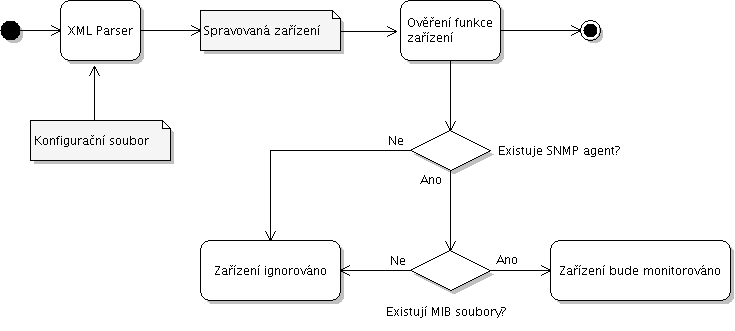
\includegraphics[width=15cm]{obrazky/05_inicializacni_faze.png}
		\caption{Inicializační fáze}
		\label{obr_impl_inicializacni_faze}
	\end{center}
\end{figure}

Po zpracování údajů o všech zařízeních, inicializační fáze končí a systém započne fázi transformační.

\subsection{Transformační fáze}
V této chvíli přebírá úlohu třída \textit{\textbf{Mib2Xsd}}, která se stará o převod MIB popisu databáze do XSD formátu. Pro manipulaci se SNMP je
použita knihovna \textit{\textbf{net-snmp}}. %TODO: citace zdroje netsnmp

Samotný převod a generování XSD popisu je rekurzivní sestup po jednotlivých uzlech virtuálního stromu MIB databáze.

Pro každé zařízení systém načte všechny specifikované MIB soubory a započne s transformací. Proces se řídí pravidly, které byly definovány v kapitole \ref{kap_xml}.
Jednotlivé uzly jsou popsány svým typem, který obsahuje jejich unikátní identifikační číslo (OID), typ dat a přístupová práva. Samotné uzly jsou pak zařazeny
do stromové hierarchie v rámci dokumentu.

Informace vztahující se k jednotlivým zařízeními jsou generovány do oddělených souborů. Samostatný soubor
pak obsahuje schéma brány a pouze identifikaci spravovaných zařízení. Tento systém byl vytvořen pro ušetření komunikační zátěže mezi manažerem a bránou.
Bližší popis výhod tohoto přístupu dále v této kapitole.

Oproti navrženému systému mapování MIB do XSD (\cite{macejko_dipl}) byla vynechána nutnost použítí prostorů jmen pro jednotlivé MIB databáze. Vzhledem
k tomu, že každý element je popsán unikátním jménem a OID, nedojde při zpracování požadavků ke konfliktu.

Abychom ušetřili procesorový čas, je paralelně s generováním schématu vytvářen i XML dokument, který za běhu slouží k vyhledávání a ostatním potřebným
operacím. Oproti schématu vypadá element specifikující uzel v MIB databázi jako na obrázku \ref{obr_impl_xml_element}.
\begin{figure}[htp]
	\begin{center}
		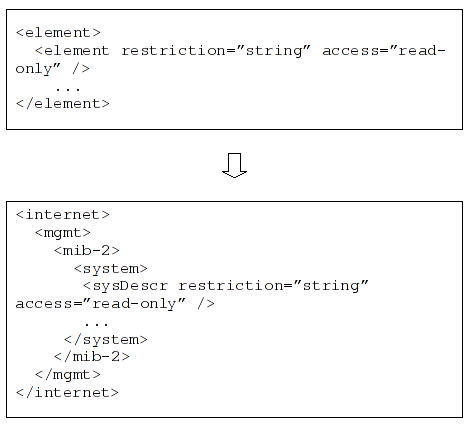
\includegraphics[height=10cm]{obrazky/05_element_xml.png}
		\caption{Příklad struktury hlavního XML dokumentu}
		\label{obr_impl_xml_element}
	\end{center}
\end{figure}

Tento dokument je pak spravován a využíván třídou \textit{\textbf{XmlModule}}.


\subsection{Komunikační moduly}
Po úspěšném zpracování a trasformaci MIB databází je možné přistoupit k inicializaci komunikačních jednotek a otevření síťových spojení k bráně.
V této fázi předává třída \textit{ \textbf{SnmpXmlGate} } řízení třídám \textit{ \textbf{SnmpModule} } a \textit{ \textbf{XmlModule} }. Tyto
moduly pak zajišťují kompletní provoz protokolové brány.

\subsubsection*{XmlModule}
\label{kap_impl_xmlmod}
Dle návrhu programu v kapitole \ref{kap_analyza} bylo uvedeno, že pro komunikaci mezi bránou a manažery bude použit HTTP server zabudovaný do
aplikace, abychom měli větší kontrolu nad posílanými daty. Proto byl použit nejvhodnější kandidát - microHTTP server %TODO cite reference na libmicrohhtpd.
Tento server je napsán v jazyce C a velice dobře posloužil našemu účelu. 

Jednotlivá spojení jsou zpracovávána samostatnými vlákny, aby bylo zaručeno co nejrychlejší odbavení požadavků. Funkční cyklus vlánka je znázorněn
na schématu \ref{obr_impl_xmlmod_vlakno}. 
\begin{figure}[htp]
	\begin{center}
		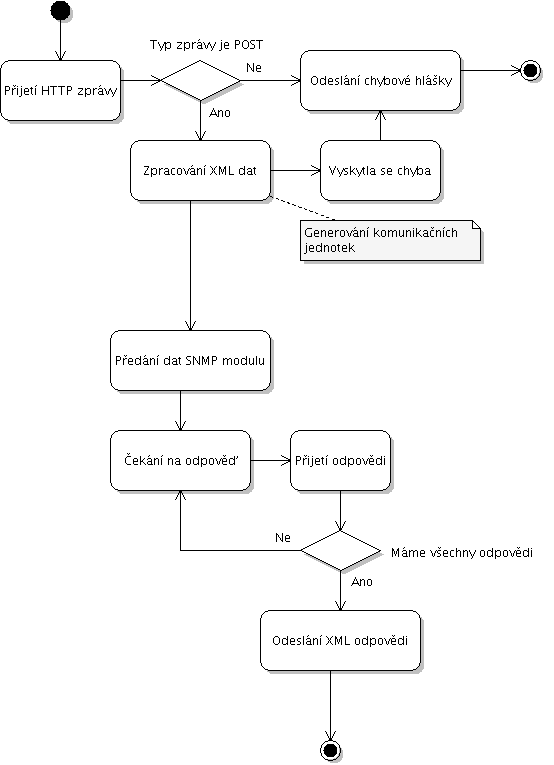
\includegraphics[width=13cm]{obrazky/05_xmlmod_vlakno.png}
		\caption{Zpracování manažerského požadavku}
		\label{obr_impl_xmlmod_vlakno}
	\end{center}
\end{figure}

Nejprve je zpracována HTTP zpráva. Systém operuje pouze s HTTP zprávami typu POST. Jakékoliv GET zprávy jsou zahazovány a zpět klientovi je zasláno
chybové upozornění. Poté je na data použit XML parser, který zpracuje požadavek a ujistí se, že je ve formátu specifikovaném v kapitole \ref{kap_xml}.
Všechny zprávy jsou zpracovávány najednou, aby byla zaručena integrita dat a "atomicita" operací. Více v kapitole \ref{kap_impl_fronta_atomicita}. 
Přesné zpracování jednoho požadavku je popsáno dále v této kapitole.

Pro komunikaci vláken s druhým modulem byly vytvořeny fronty požadavků (pro směr od XML modulu k SNMP modulu)
a jedna odpovědní fronta, ze které se poté vybírají vyřízené požadavky.
Když jsou všechny zprávy v pořádku zpracovány, jsou odeslány do fronty k příslušnému monitorovanému zařízení, nebo jsou rovnou zařazeny
jako odpovědi (obsahují-li chybu, která znemožňuje její další zpracování). Zařazení do fronty k vláknu má na starosti SNMP modul a zároveň
i on probouzí příslušné vlákno ke zpracování požadavků.

Vlákno se následně přesune do čekajícího cyklu, kde kontroluje odpovědní frontu na svoje požadavky do doby, než se dostaví všechny odpovědi. 
Poté vygeneruje odpovědní zprávu a zašle manažerovi. Tím jeho životní cyklus prakticky končí. Je na serveru, jak s vlákny poté naloží a jak 
je recykluje. Takzvané zamrznutí a nekonečné čekání vlákna je ošetřeno maximální prodlevou pro jeden požadavek v SNMP modulu. Tím je zaručeno, že
manažer určitě dostane odpověď.

\subsubsection*{Jednotka komunikace}
Než přistoupíme k popisu zpracování jednotlivých XML zpráv, je důležité popsat, jak spolu komunikují oba moduly. Z navrženého protokolu jasně 
vyplývá, že XML manažer komunikuje s bránou tak, jako by to byl samotný XML agent. O protokolu SNMP nesmí vědět. Proto byl již při návrhu
brán zřetel na striktní oddělení těchto dvou protokolů. Pro komunikaci byla navržena struktura, která v sobě obsahuje veškeré informace o
požadavku a odpovědi, ale je protokolově neutrální.

Důležité položky struktury, které oba moduly využívají jsou:
\begin{itemize}
	\item \textbf{typ zprávy} - definuje, jaký požadavek byl vyslán (Get, Set). Dle toho se pak vytvářejí SNMP požadavky na agenta.
	\item \textbf{seznam uzlů} - seznam dvojic (jméno, hodnota), které manažer požaduje.
	\item \textbf{chyba} - identifikace a textová reprezentace chyby, která v celém zpracujícím procestu nastala.
\end{itemize}

Tato struktura pak obsahuje informace o jednom požadavku (Get, Set, Subscribe), který byl v XML zprávě obsažen. 


\subsubsection*{SnmpModule}
Komunikace se SNMP agentama je založen na systému front. Každé monitorované zařízení má na straně protokolové brány k dispozici jedno obslužné vlákno
a frontu zpráv. Schématicky naznačeno na obrázku \ref{obr_impl_snmp_komunikace}. Zpracování a vytváření SNMP zpráv se děje pomocí knihovny \textbf{net-snmp}.
\begin{figure}[htp]
	\begin{center}
		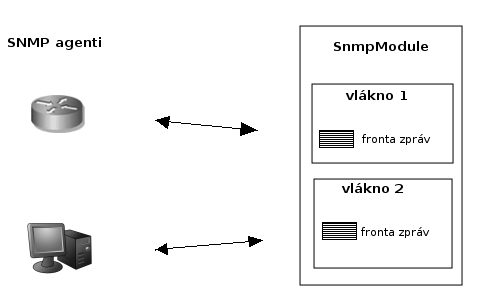
\includegraphics[width=14cm,height=8cm]{obrazky/05_snmp_komunikace.png}
		\caption{Komunikační vlákna brány pro spojení se SNMP agenty}
		\label{obr_impl_snmp_komunikace}
	\end{center}
\end{figure}

Práce komunikačních vláken probíhá v "nekonečném" cyklu. Vstupní informací pro vlákno je identifikační
číslo monitorovaného zařízení, ke kterému patří. S touto informací získá přístup k frontě zpráv a dalším potřebným strukturám, příslušející pouze danému agentovi.
V cyklu se pak opakuje několik dílčích bloků stále dokola.

Vlákno zjistí, jestli v příslušné frontě je přítomen nějaký požadavek na vyřízení. Když není, vlákno se uspí. Jinak vyjme všechny dotazy, tím frontu vyprázdní a
požadavky zpracuje. Tento funkční blok závisí na typu zprávky, která se má vyřídit. 

Zprávy Get a Set, které mají za úkol dostat nebo nastavit hodnotu koncového uzlu stromu, plně korespondují se SNMP. Je vytvořen SNMP packet, do kterého je vloženo
heslo (community string) na základě přístupových práv, které manažer má, je naplněno daty, které se mají nastavit či získat a dotaz je odeslán.

Po přijetí odpovědi jsou data opět z paketu vyjmuta, upravena do požadovaného formátu v rámci komunikační struktury. Pakliže se vyskytla chyba při zpracování, opět
je nastaven příznak ve struktuře, aby manažer dostal informace o problému. Takto vygenerovaná odpověď je poslána do odpovědní fronty a je probuzeno vlákno, které na
data čeká (samotná funkce je ve správě XML modulu).

Složitější je zpracování požadavku na uzel, který není koncový a obsahuje pod sebou celý podstrom dalších uzlů (z hlediska MIB databáze). Poté je nutno opakovat
vytváření paketů a zasílání dotazů ve formě SNMP zprávy GetNextRequest. Až poté, co jsou získána všechna data, je navrácena odpověď klientskému vláknu v XML modulu.


\subsection{Zprávy}
Zpracování jednotlivých druhů zpráv se odvíjí od navrženého modelu. Následuje popis chování systému při přijetí jednotlivých požadavků.

\subsubsection*{Discovery}
Jediným omezením při zpracování požadavku je verze XML protokolu, kterou manažer posílá ve zprávě. Když se rozchází s nastavenou 
verzí v systému, odpovědí je zpráva Publication a chybové hlášení.

Jedním z implementačních požadavků bylo též snížit množství dat mezi manažerem a bránou. Předpokládáme, že brána spravuje
desítky SNMP zařízení. Celý dokument, popisující všechny informace, který je odpovědí na tento požadavek by pak nabyl
obrovských rozměrů. Pro zlepšení protokolu tak systém zašle manažerovi pouze hlavní popis brány s identifikací jednotlivých zařízení, bez ostatních dat.
Manažer si může vybrat, které zařízení chce spravovat a zašle novou zprávu Discovery s volitelným atributem \textbf{objectid}. Po zpracování
mu brána zašle pouze XSD dokument popisující právě to jedno zařízení.

\subsubsection*{Get a Set}
Zpracování těchto požadavků prochází několika fázemi v rámci samotného XML modulu.

Nejprve je nutné zjistit, jestli má manažer právo tyto operace provádět. Heslo, které se zasílá v elementu \textit{message}, určuje, jestli je
povoleno čtení, či zápis. Nastavení hesel probíhá při inicializační fázi a tyto jsou čtena z konfiguračního souboru. Celý přístupový model je
založen na dvou heslech XML protokolu - pro čtení a zápis. Každé SNMP zařízení má pak definovány opět dvě hesla, která jsou odlišná od těch prvních jmenovaných.
Systém pak na základě dodaného XML hesla zjistí, jaké má uživatel práva a použije pak příslušné SNMP heslo pro požadavek. Může se stát, že mangažer zadal
špatné heslo a systém mu přístup odepře. Pak je odpovědí na tyto požadavky chybová zpráva.

Když uživatel má dostatečné oprávnění, je nutné zjistit, zda-li uzly, na které se dotazuje, opravdu existují. Dotazování probíhá pomcí jazyka XPath.
Pakliže je dotaz špatně formulován, nebo element neexistuje, systém požadavek zamítne. V druhém případě mohou nastat dvě eventuality.

Element je koncovým uzlem stromu, tj. obsahuje pouze hodnotu danou definovaným typem. Systém takový dotaz interpretuje jako jediný SNMP dotaz GET.
Když se ale jedná o kořenový uzel (obsahuje podstrom uzlů), je nutné tento dotaz interpretovat jako
SNMP zprávu GETNEXT a získat všechny hodnoty daného podstromu (o což se stará SNMP modul).

Jestli bylo požadavkem nastavení určité hodnoty, pak je součástí datové struktury jméno uzlu a příslušná hodnota.

Vygenerovaná komunikační jednotka je vložena do fronty požadavků a pak současně se všemi ostatními odeslána SNMP modulu ke zpracování.

\subsubsection*{Subscribe}
Touto zprávou se manažer upisuje k zasílání pravidelných informací o daném agentovi, nebo tyto údaje mění a maže. Každý takový záznam
se zanese do hlavního XML dokumentu, aby bylo při úpravách a mazání možné vyhledávat pomocí XPath výrazu. Reakce na přidání a úprava
vnitřních struktur je ponechána na speciální vlákno, které slouží k obsluze daných záznamů. Bližší specifikace dále v této kapitole.

Jediný problém při implementaci nastal v rámci mazání jednotlivých záznamů. Vzhledem k tomu, že v navrženém protokolu je odpovědí
manažerovi zpráva Distribution s daty, která požaduje, nebo chyba, je nutno při smazání záznamu poslat opět zprávu Distribution, ale nyní
prázdnou.

Práva k mazání a úpravám daného záznamu jsou ponechána pouze na znalosti unikátního identifikátoru. 


\subsubsection*{Změny oproti navrženému XML protokolu}
Oproti navrženému XML protokolu bylo nutno udělat několik drobných změn, abychom mohli celý systém implementovat. Jedná se pouze o
minoritní změny - přidání volitelného atributu \textbf{objectid} ke všem typům požadavků, které manažer zasílá. Je to z důvodu
identifiace monitorovaného zařízení, což by bez tohoto zásahu nebylo vůbec možné. Zároveň tento zásah umožňuje ponechat stejnou
strukturu protokolu (co se týče dotazů a odpovědí) pro stroj agenta a brány. 

Abychom nezměnili dosavadní protokol, byl tento atribut zvolen jako volitelný. Jeho nepřítomnost signalizuje, že dotaz je mířen
na samotné zařízení brány, která následně přepošle požadavek na SNMP agenta běžícího na tom samém stroji.


\subsection{Fronty a atomicita požadavků}
\label{kap_impl_fronta_atomicita}
Systém předávání požadavků pomocí front vychází z navrženého protokolu (\cite{macejko_dipl}), ale byl přepracován pro potřeby
této protokolové brány. Navrhovány byly fronty, které by zpracovávaly požadavky dle priority a mamažer by si mohl říci, které
dotazy budou mít jakou prioritu. To bohužel zcela nevyhovuje požadavku zajištění posloupnosti provádění dotazů a tím pádem i 
integritě dat.

Předpokládejme situaci, kdy manažer v jedné XML zprávě zašle dotaz na hodnotu jednoho uzlu s nižší prioritou a zároveň také nastavení
jiné hodnoty s vyšší prioritou (viz obrázek \ref{obr_impl_atom1}). Stalo by se, že při zpracovávání se nastavení provede dříve a manažer by se nikdy nedozvěděl starou hodnotu.
\begin{figure}[htp]
	\begin{center}
		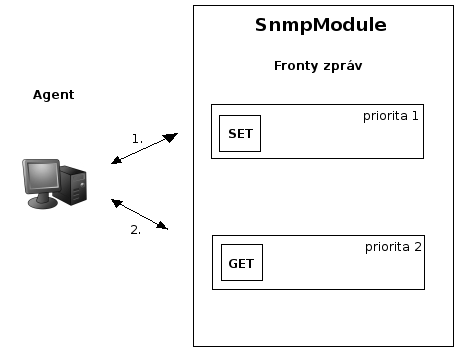
\includegraphics[width=10cm]{obrazky/05_atom1.png}
		\caption{Chyba prioritního zpracování požadavků}
		\label{obr_impl_atom1}
	\end{center}
\end{figure}

Druhým problémem je "atomicita" prováděných operací. Kdyby systém zpracovával jeden požadavek z přijaté zprávy, čekal na odpověď agenta, a pak
přešel na další, mohlo by se stát, že druhý manažer by mohl do tohoto cyklu vstoupit a narušit tak výsledek celé posloupnosti operací.

Proto byl systém přepracován tak, že každé monitorované zařízení má v SNMP modulu jedno obslužné vlákno a frontu požadavků (jak bylo vysvětleno 
dříve v této kapitole). Nyní se v XML modulu zpracují všechny požadavky v rámci jedné zprávy, vygenerují se příslušné komunikační struktury a ty jsou
následně všechny najednou vloženy do příslušné fronty požadavků. Tato funkce je ponechána na SNMP modulu, který zajistí, pomocí systému výlučného přístupu
k dané frontě, aby všechny zprávy tvořily souvislý blok, který bude sekvenčně zpracován.

Je možné, že uživatel v rámci jedné zprávy zašle dotazy na více zařízení. Každé takové zařízení obdrží svůj blok dotazů individuálně.

Předávání odpovědí ze SNMP do XML modulu slouží pouze jediná odpovědní fronta. Do ní se vkládají postupně vyřízené požadavky ze všech zařízení.
Vždy, když je vložena odpověď, jsou probuzena klientská vlákna, zkontrolují frontu a případně si vyberou jim určené odpovědi. Zde by se mohlo zdát,
že bude narušena posloupnost jednotlivých odpovědí v případě, ze komunikujeme s více zařízeními. Tento fakt je ošetřen unikátním identifikátorem každého
požadavku v zasílané zprávě. Odpovědi poté obsahují stejný identifikační řetězec, díky kterému pak manažer pozná, k jaké zprávě se vztahuje obdržená hodnota.

\subsection{Periodické zasílání informací}
Jednotlivými zprávami typu Subscribe se manažer upíše k pravidelnému zasílání informací. Tuto činnost zahrnuje v sobě XML modul, kde na obsluhu těchto
rozesílání je vyhrazeno speciální vlákno. To se stará o veškeré manipulace s jednotlivými záznamy, získávání informací od agentů (pomocí SNMP modulu) a jejich
předávání dále.

Celý systém správy záznamů je založen na hlavním XML dokumentu. Každé spravované zařízení má ve své části element \textit{subscriptions}, kam jsou ukládány
informace o jednotlivých manažerech. Jeden příkladný záznam je schematicky vyjádřen na obrázku \ref{obr_impl_subscript_element}.
\begin{figure}[htp]
	\begin{center}
		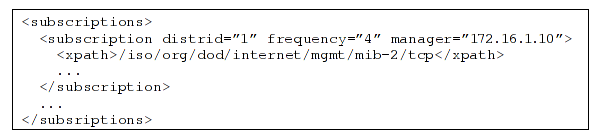
\includegraphics[width=14cm]{obrazky/05_subscr_element.png}
		\caption{Element subscription v rámci hlavního XML dokumentu}
		\label{obr_impl_subscript_element}
	\end{center}
\end{figure}

Každý záznam je identifikován jedinečným číslem a zároveň i zařízením, ve kterém se nachází. Dále element subscription obsahuje informace o frekvenci zasílání, 
url manažera, kam se mají pakety doručovat a v poslední řadě jsou to jednotlivé XPath výrazy pro identifikaci uzlů z databáze dat.
Veškeré úpravy - přidávání, změna a mazání - jsou ponechány ve správě tohoto vlákna.

\subsubsection*{Přidání záznamu}
Když manažer zašle požadavek na zapsání, je obsluhujícím vláknem vytvořen nový element \textit{subscription}, naplněn daty, umístěn do XML dokumentu a 
distribuční vlákno je upozorněno, že nastala změna. Jsou prohlédnuty všechny záznamy a vygenerovány interní datové struktury pro další správu.

\subsubsection*{Úprava záznamu}
Vlákno, které zpracovává požadavek klienta, upraví daný záznam v XML dokumentu a oznámí distribučnímu vláknu změnu. To se pak, identicky jako v předchozím případě,
přesvědčí, jaké změny nastaly a upraví interní data.

\subsubsection*{Smazání záznamu}
Záznam, pakliže existuje, je označen jako smazaný, ale vlastní smazání provádí až distribuční vlákno.

\subsubsection*{Zasílání informací}
Vlastní zasílání informací probíhá v jednoduchém cyklu. Jestli není jediný záznam k dispozici, vlákno se uspí a čeká na příchozí zprávy Subscribe. Jsou-li záznamy
k vyřizování, zvolí se nejmenčí časový krok, který je nutný čekat (dle frekvence zasílání jednotlivého záznamu) a vlákno se uspí. Po probuzení je odečten
prospaný čas ode všech záznamů a u těch, které jsou připraveny k vyřízení, předá distribuční vlákno připravené komunikační jednotky SNMP modulu, pro vyřízení
vlastní komunikace. Poté, co dostane odpověď, inicializuje spojení pomocí knihovny \textbf{\textit{libCUrl}} a zprávu Distribution zašle manažerovi na příslušnou
adresu.

Pakliže zpráva nedojde z jakéhokoliv důvodu - manažer je vypnutý, nemůže být zahájeno spojení - je započítán neplatný pokus o odeslání. V momentu, kdy tento počet
překročí stanovenou hranici, je daný záznam smazán a manažer bude muset požádat o nové zapsání zprávou Subscribe. Tento systém je zvolen pro zamezení zahlcení 
distribučního vlákna, které by pak v extrémním případě mohlo spravovat desítky až stovky nefunkčních záznamů, které si nikdo nevyzvedne.


\subsection{Asynchronní události}
Přijímání a zpracování veškerých asynchronních událostí, které agenti posílají na protokolovou bránu, má za úkol speciální vlákno ve správě SNMP modulu.
Funkce tohoto vlákna je přijmout SNMP zprávu (Trap, Notification), zjistit o jaké zařízení se jedná, zvolit všechny manažery, kteří jsou nastaveni pro příjem
XML zprávy Event a zprávu odeslat.

Veškeré nastavení monitorovaných zařízení z hlediska příjemců těchto zpráv je v konfiguračním souboru. Při inicializaci vlákna je zpracován tento seznam pro každé
zařízení.

Vlákno se pak přesune do nekonečného cyklu, kde čeká na definovaném portu na příjem zprávy. Příjem a získání SNMP paketu z příslušného datového spojení je ponecháno
na knihovně \textbf{\textit{net-snmp}}.

Samotné zpracování pak v sobě zahrnuje získání informací o události, inicializaci jednotlivých spojení pomocí knihovny \textbf{\textit{libCUrl}} a zaslání XML zprávy
Event jednotlivým manažerům. Z navrženého protokolu vyplývá povinnost získat potvrzení o doručení paketu. To za nás vykoná transportní protokol TCP, který je knihovnou libCUrl
použit. Není-li možné paket doručit - manažer neexistuje či je vypnutý - pak je informace zahozena a brána se již o tento fakt nezajímá.


\section{Paměťové optimalizace}
Hlavním bodem zadání této práce není jenom implementace protokolové brány, ale i optimalizace využití operační paměti. Při vývoji se objevily dva body, kdy bylo nutno 
vymyslet optimalizaci systému. Oba dva body se opírají o manipulaci a uložení XML dokumentů, které v paměti zabírají velký prostor.

Prvním je správa XSD schémat, která popisují jednotlivá monitorovaná zařízení. Každou příchozí zprávou Discovery se manažer dotazuje na tyto popisná schémata. Bylo by, pro 
rychlejší odbavení požadavku, snadnější uchovávat celá schémata v paměti. Za předpokladu, že jedno schéma zabírá minimálně několik stovek kB (při použití pouze standardní
sady MIB databáze) paměti a že bychom spravovali několik desítek zařízení, mohla by se nutná paměť rozrůst do desítek MB. Proto se každé takovéto schéma ukládá do
souboru na pevném disku a v případě potřeby je soubor načten a zaslán manažerovi. Časový rozdíl je relativně malý v porovnání s množstvím paměti, která se ušetří.

Druhým bodem je minimalizace velikosti hlavního XML dokumentu, který je udržován po celou dobu chodu protokolové brány v paměti. Není dost dobře možné, bez zásadních změn
navrženého protokolu, sdílet části virtuálního stromu dat. Proto vycházejme z předpokladu, že na spravované síti reálně existují identická zařízení, která používají
stejnou sadu MIB databází. Zároveň je tu druhý předpoklad, že v rámci běžné sítě se nepoužívá mnoho jednotlivých zařízení, která by v rámci SNMP protokolu nabízela ke správě odlišná data.
Kdybychom měli u každého takového zařízení spravovat v hlavním XML dokumentu celý datový strom, nebylo by možné udržet tento v paměti a zároveň na něm provádět
efektivně vyhledávání a jiné operace.

Proto byl stanoven takzvaný sdílený systém, který se dotýká i prvního bodu. Zařízení, která mají v konfiguračním souboru nastavenu stejnou sadu MIB databází, jsou prohlášena za shodná, co se týče
dat, a je vytvořeno pouze jedno popisné XSD schéma a do hlavního dokumentu je uložen pouze jeden takovýto strom. Ostatní zařízení mají nastaveno identifikační číslo shodného agenta.
Při jakémkoliv požadavku na vyhledání elementů ve stromu či popisné schéma, je vyhledáváno právě v tom jediném sdíleném stromu, nebo navráceno jediné sdílené schéma.

Tímto nejenom, že v rámci předpokladů ušetříme aktuální operační pamět, ale zároveň i místo na pevném disku, kde jsou popisná schémata ukládána. Z hlediska splnění zadání bylo tedy
dosaženo optimálního řešení.


\section{XML Manažer}
Nedílnou součástí implementační části je vytvoření XML manažera, který by dovolil otestovat protokolovou bránu v praxi. Vzhledem k tomu, že není náplní práce vytvořit plnohodnotného
klienta, který by postkytoval veškeré uživatelské pohodlí grafické aplikace a jiných možných aspektů, byl vývoj omezen na tvorbu aplikace ovládané pomocí příkazového řádku.

K tvorbě manažerské aplikace byly použity knihovny:
\begin{itemize}
	\item \textbf{ \textit{libCUrl} } - zajištující klientské spojení s HTTP serverem na bráně
	\item \textbf{ \textit{libMicroHTTPD} } - HTTP server použitý pro příjem asynchronních událostí a periodiské distribuce dat
	\item \textbf{ \textit{libargtable2} } - knihovna zajišťující pohodlnné zpracování vstupních parametrů programu
\end{itemize}

Aplikace funguje ve dvou možných formách - aktivní nebo pasivní (kompletní instalační a uživatelská příručka je v příloze \ref{kap_uzivatelska_prirucka_manazer}).

\subsubsection*{Aktivní mód}
V tomto módu je součástí vstupních parametrů URL protokolové brány, XML heslo a soubor, který obsahuje jednotlivé požadavky, které chce
uživatel provést. Systém načte vstupní soubor a pakliže je vše bez chyby zpracováno, vygeneruje XML zprávu dle navrženého protokolu. 

Tuto zprávu pak odešle a čeká na odpověď. V případě, že byla odeslána zpráva Subscribe a jsou tedy očekávány periodické dodání informací,
je spuštěn HTTP server a jako v předchozím případě, aplikace čeká na odpovědi.

Při ukončení tohoto čekání zašle aplikace XML zprávu, kterou zruší veškeré Subscribe záznamy, které předtím odeslala.

\subsubsection*{Pasivní mód}
Tento mód slouží jako takzvaný "poslouchací". Při něm se pouze aktivuje webový server a očekávají se příchozí zprávy ohledně asynchronních událostí.
V tomto módu nelze odesílat žádné požadavky.


%seznam literatury
\bibliographystyle{abbrv}
\bibliography{reference.bib}

\end{document}
